\chapter{Implementation}
This chapter is concerned with the implementation details of the individual components introduced in Chapter \ref{chapter:4}. This includes the development of the Unity application responsible for producing the front-facing camera video stream and displaying the visual cues, the development of the human detection and direction system, as well as the reactive control systems implemented on ARTA. Previous work in the PRL had utilized the Hololens camera to capture images that were then processed on an external computer, but where this project differs is that a video stream is required to perform real-time object detection. As such, a large amount of time was spent at the very beginning of the project trying to produce a video stream, since the whole project depended on this form of visual input.

\begin{figure}[ht]
	\centering
	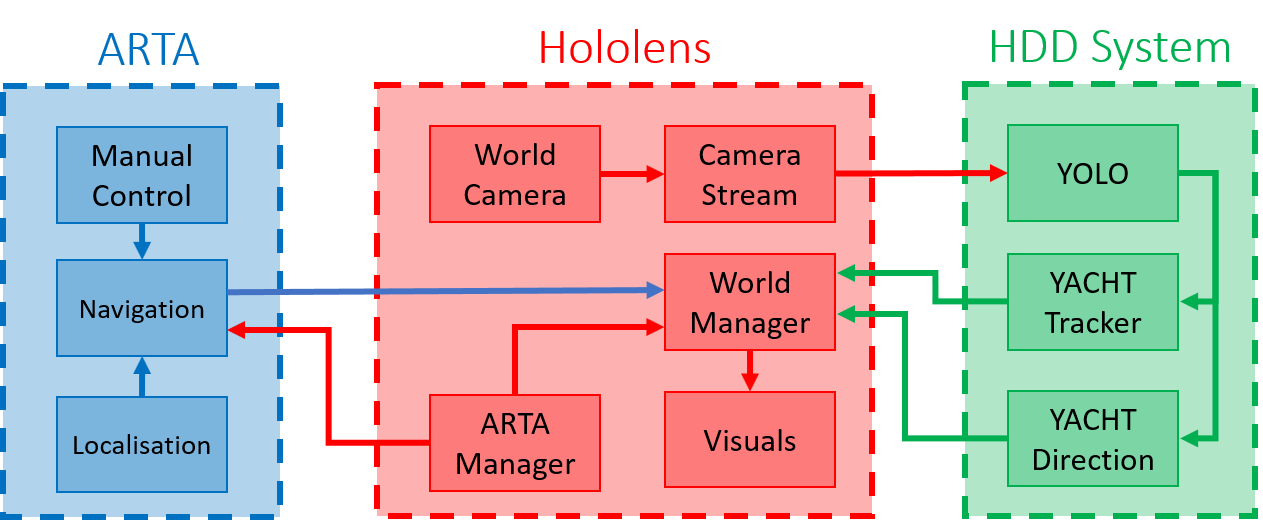
\includegraphics[width=1.0\linewidth]{img/chapter5_implementation/detailedSystemDiagram.png}
	\caption{System diagram detailing individual components of the programs running on each device.}
	\label{fig:detailedHL}
\end{figure}

Figure \ref{fig:detailedHL} is a more detailed diagram of the high level system digram presented in Figure \ref{fig:simplifiedHL}. We show the communication between the three separate devices, and how each node can be broken down into smaller nodes running specific computations. For the rest of this report, we represent the ARTA, Hololens and HDD system components with the colours blue, red and green respectively.

\section{Human Detection \& Direction System}
In order to determine the direction people are walking in, it is necessary for the system to be able to detect humans. Only after detection is it possible to discern the motion of individuals, which can be achieved through object tracking and body pose estimation. Figure \ref{fig:detailedHDD} shows the breakdown of the HDD node into components responsible for these two tasks. This section is concerned with the implementation of the methods needed to perform the direction prediction, as well as how the system communicates between its nodes. 

\begin{figure}[ht]
	\centering
	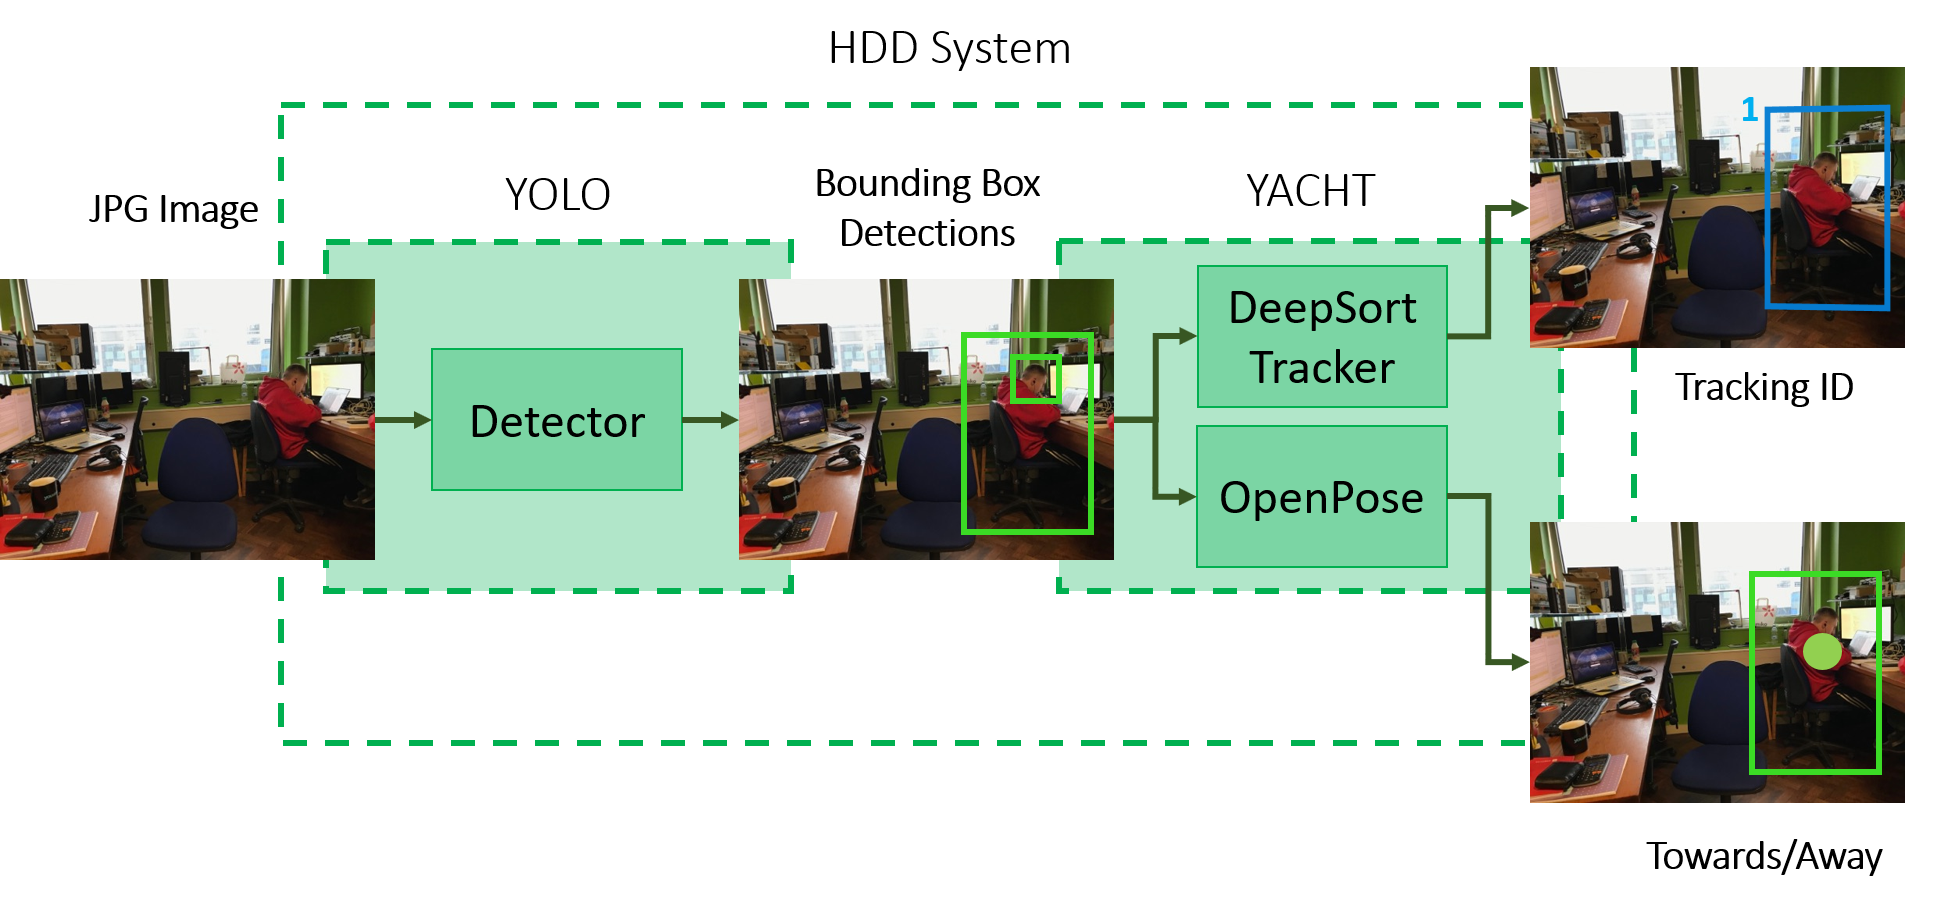
\includegraphics[width=1.0\linewidth]{img/chapter5_implementation/hddSystemDiagram.png}
	\caption{The HDD System is sub-divided into two ROS packages, YOLO and YACHT. We show that YACHT has two sub-nodes which both depend on the outputs of the detector.}
	\label{fig:detailedHDD}
\end{figure}

We begin this section by listing the hardware requirements for the system. Due to the nature of the HDD, and its reliance on modern deep learning techniques, access to a modern GPU is essential. We refrain from trying to explain the step-by-step process to setup the hardware and software, and instead point the reader in the direction of an article\footnote{https://link.medium.com/xQ5w2FMXoX} which covers this topic.

\subsection{Hardware \& Software Dependencies}

\subsubsection{Hardware}
We implemented the HDD system on a desktop computer connected to the Imperial College network. Due to the real-time computer vision requirements of this project, the computer was chosen due to the GTX 1050Ti GPU with 4GB video RAM available on the system. The computer was also equipped with an Intel i7-2600 CPU and 8GB DDR3 RAM.

\subsubsection{Software}
We have refrained from posting all Python dependencies for the project and only mention the key ones. A complete listing is available in the appendix. The following software dependencies are required to run this project:
\begin{itemize}
	\item Ubuntu 16.04
	\item Python 2.7
	\item OpenCV 3.0
	\item ROS Kinetic
\end{itemize}

Due to the deep learning component of the project, the following software dependencies are essential:
\begin{itemize}
	\item Nvidia Graphics Drivers 
	\item CUDA 8.0 Toolkit
	\item cuDNN 6.0
	\item Darknet
	\item Tensorflow-GPU
	\item Caffe
\end{itemize}

\subsection{YOLO Object Detector}
As mentioned in Section \ref{sec:yolo}, we chose to use the YOLOv3 Tiny architecture and trained it on the CrowdHuman dataset. We begin this section by introducing the reader to \textbf{Darknet}, the neural network framework YOLO is implemented on, and how we integrated it into ROS. We also briefly explain how the network detects objects, and compare YOLOv3-tiny with the more memory intensive YOLOv3. We then guide the reader through the training process, and the analysis we did to validate the human detection improvements compared to pre-trained models.

\subsubsection{Darknet}
Darknet\footnote{https://pjreddie.com/darknet/} is an open source neural network framework written in C and CUDA which supports both CPU and GPU computation \cite{darknet13}. The source code for the framework is freely available on GitHub, and it can be used to train different neural network architectures in a manner similar to more conventional deep learning frameworks such as Tensorflow or Caffe.

\subsubsection{Darknet in ROS}
By definition, ROS is language-independent, although at the time of writing, three main libraries have been defined for ROS, making it possible to program ROS in Python, Lisp or C++. On the other hand, Darknet is implemented in C, due to the speed of compiled low-level languages in conjunction with CUDA. However, the Darknet framework is compiled into \textit{Shared Object (.so)} file, which is analogous to a Windows DLL. As such, it becomes possible to access the framework by writing wrappers around the compiled library file.

\paragraph{}Darknet has basic Python wrappers around the compiled library which convert Python data types into C and vice versa. However, the original wrappers for detection are written to run on images that are saved on disk. Darknet converts the saved images into a C data structure \code{IMAGE} and performs the detections. To integrate the framework into ROS, the node must be able to receive data from image topics with \code{CompressedImage} or raw \code{Image} messages.

\paragraph{}In ROS Python, the JPG or PNG images received from the \code{CompressedImage} message can be converted to numpy arrays which store the RGB values, without the need to be saved on disk. As such, we wrote Python wrappers for Darknet that allow the framework to support images in the form of numpy arrays as well as images saved on disk. The following listing defines the \code{IMAGE} data structure, and the conversion of an image numpy array to the Darknet format: \\



\begin{lstlisting}[language=Python, caption={Darknet IMAGE Python wrappers for seamless ROS integration.}]
# IMAGE: a C data structure used by Darknet
class IMAGE(Structure): 
	_fields_ = [("w", c_int),
				("h", c_int),
				("c", c_int),
				("data", POINTER(c_float))]
				
# Converts numpy array to Darknet IMAGE type
def nparray_to_image(img): 
	data = img.ctypes.data_as(POINTER(c_ubyte))
	image = ndarray_image(data, img.ctypes.shape, img.ctypes.strides)

	return image
\end{lstlisting}

Further Python wrappers were written for the detection and return of the image bounding box co-ordinates. We also created ROS messages for the bounding box detections, which allows the Darknet YOLO node to communicate with other nodes in the HDD system. The full code listing can be found in the Appendix \footnote{https://github.com/alaksana96/darknet-crowdhuman}\footnote{https://github.com/alaksana96/fyp\_yolo}.

\subsubsection{YOLO Detection Algorithm}
As researched in Section \ref{sec:backYOLO}, the algorithm divides an input image into an $S\times S$ grid. Each grid cell can predict one object, and a cell can predict a fixed number of bounding boxes $B$, which we visualize in Figure \ref{fig:yoloViz}. The predicted bounding box is chosen from the set of $B$ boxes with the highest box confidence score, which is a measure of how likely the box contains an object and how accurate the boundary box is. It also predicts the conditional class probability, which is the probability a detected object belongs to a certain class. 

\begin{figure}[ht]
	\begin{subfigure}[b]{.45\textwidth}
		\centering
		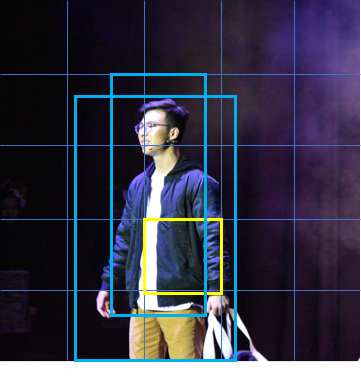
\includegraphics[width=1.0\linewidth]{img/chapter5_implementation/yoloAlgo1.png}
		\caption{A grid cell can make $B$ predictions, in this example $B=2$.}
	\end{subfigure}%
	\hspace{\fill} 
	\begin{subfigure}[b]{.45\textwidth}
		\centering
		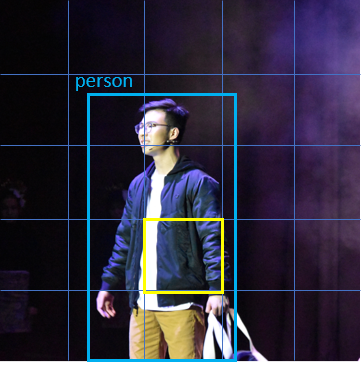
\includegraphics[width=1.0\linewidth]{img/chapter5_implementation/yoloAlgo.png}
		\caption{The bounding box with higher box confidence score is used.}
	\end{subfigure}
	\vspace{-1\baselineskip}
	\begin{center}
		\caption{Visualization of the YOLO person detection algorithm dividing a resized square image into grid cells.}
		\label{fig:yoloViz}
	\end{center}
	\vspace{-2\baselineskip}
\end{figure}

\subsubsection{YOLOv3 Tiny vs YOLOv3}
While testing out the different models, we noticed that the YOLOv3 model was consistently crashing and causing segmentation faults. On further investigation, we noticed that this was due to the network using up all 4GB of video memory available on the GPU. In comparison to its predecessors YOLO and YOLOv2, YOLOv3 is a much larger network which has 106 fully convolutional layers. Although it is far more accurate at predicting bounding boxes, it reduces the frame rates that can be achieved on video. As such, we decided to use YOLOv3 Tiny, a shallower variant of the network that is suitable for real-time image detection. Although the tiny version is not as accurate, it is much lighter on memory, using less than 1GB video RAM, making it a suitable choice for this project.

\subsubsection{Training YOLOv3 Tiny}
\paragraph{CrowdHuman} The CrowdHuman dataset \cite{Shao} is a benchmark dataset to better evaluate detectors in crowd scenarios. The most important features of the dataset are the size, quality of the annotations and the diversity. Each image contains multiple people with varying degrees of occlusion, which allows for object detectors to better learn the representation of obscured people. 

\begin{figure}[ht]
	\centering
	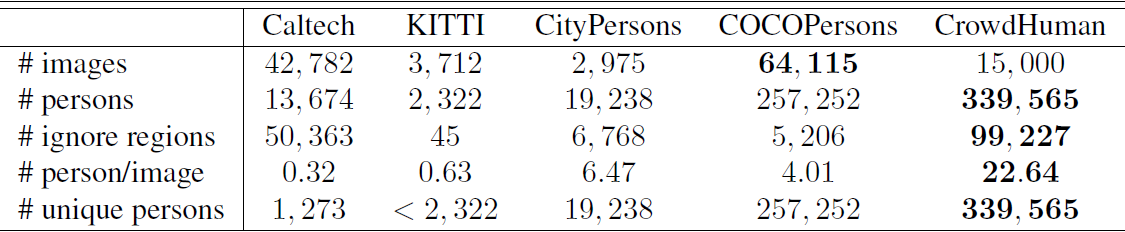
\includegraphics[width=0.9\linewidth]{img/chapter5_implementation/crowdHumanStats.png}
	\caption{A comparison of CrowdHuman to other person image datasets \cite{Shao}, showing the increase in number of people and diversity in the images.}
	\label{fig:crowdHumanStats}
\end{figure}

As can be seen from Figure \ref{fig:crowdHumanStats}, the dataset contains far more unique identities. By examining the dataset, we can see that it contains people in a wide array of situations, at varying distances with different body poses.

\paragraph{Annotations} The CrowdHuman dataset provides its annotations in the \code{.odtg} format, which is a variant of JSON. Each line in the annotation file corresponds to a JSON containing the image ID and the bounding boxes. The annotations include boxes for the \textit{visible box}, \textit{full body box} and \textit{head box}. For the purposes of this training, we chose to use the full body and head boxes only. We wanted the detector be able to learn to predict occluded individuals, and we also wanted to experiment with head pose estimation. Each bounding box is annotated as below, where \code{x,y} is the top-left corner of the bounding box. The \code{width} and \code{height} are also given in image co-ordinate pixels.

\paragraph{}\code{[x, y, width, height]}  

\paragraph{}On the other hand, to train YOLO on Darknet, the annotations must be given in a completely different format. The Darknet annotation format is as such:

\paragraph{}\code{<object-class> <x> <y> <width> <height>}

\paragraph{}Since Darknet accepts images of any size, it works with image units which are scaled relative to the size of the image. As such, all the values for the bounding boxes are between $0$ and $1$. Furthermore, the \code{x, y} values in the annotation are measured from the centre of the bounding box.  

\paragraph{Converting Annotations} To use the CrowdHuman images as a training set for the YOLOv3-tiny model, we had to write several scripts that converted the annotations to the Darknet format. We have included these scripts in the Appendix should the reader wish to convert the dataset themselves\footnote{https://github.com/alaksana96/darknet-crowdhuman/blob/master/README.md}.

\paragraph{Training Parameters} Before training, we set up the model configuration file to learn 2 classes, head and body, as well as to use batches of 32 divided into subdivision of 8 images. This limits the number of images loaded into memory at once to 8, to prevent running out of GPU memory. We also reduce the size of the training images to $416\times 416$ pixels, to further reduce the GPU usage. \\

\begin{lstlisting}[language=Mymatlab,caption={Training parameters used for YOLOv3 Tiny on the CrowdHuman dataset}]
	batch=32 %Training parameters for YOLO Tiny
	subdivisions=8
	width=416
	height=416
	channels=3
	momentum=0.9
	decay=0.0005
\end{lstlisting}

These optimizations were done in order to maximize the amount of GPU memory used for training, without a sudden surge in usage causing a segmentation fault. Resizing the input training images allows the algorithm to divide the image into a $S\times S$ grid. Generally, the larger the height and width, the better the predictions, since the image can be divided into more grid cells. This is a trade-off we had to make in order to be able to train the network on a mid-range GPU.

\paragraph{Training Process} We left the model to train overnight, creating backups of the weights every 1000 iterations. The following day, after reaching 30,000 iterations, we decided to stop training the network. The average loss error and total loss had stopped decreasing for several hours, and was hovering around $29.134$. We reasoned that the network had reached a minima, and further training would be redundant, since it would over-fit the dataset. The final weights are available in the file \code{yolov3-tiny-crowdhuman.backup} .

\subsubsection{Evaluating Trained Model}
\paragraph{Hololens Videos} As mentioned in Section \ref{sec:backYOLO}, we recorded several test videos using the Microsoft Hololens. These videos were capture in various locations on the Imperial College campus. Figure \ref{fig:yoloRange} shows the model detecting people at range.  

\begin{figure}[ht]
	\centering
	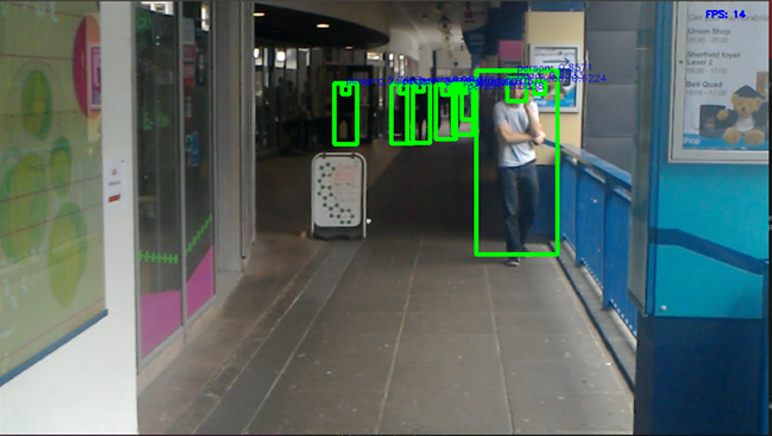
\includegraphics[width=0.5\linewidth]{img/chapter5_implementation/yoloWalkway.png}
	\caption{Trained model detects people and heads at different ranges. We also see it can detect people far away and accurately detect their heads.}
	\label{fig:yoloRange}
\end{figure}

A common area where lots of people frequent is the Sherfield walkway. As seen in Figure \ref{fig:yoloSherfield}, this was an ideal place to capture a video since it features a lot of people walking around in different directions. We captured several more videos outside the EEE building and inside the 5th floor ICRS lab.

\begin{figure}[ht]
	\centering
	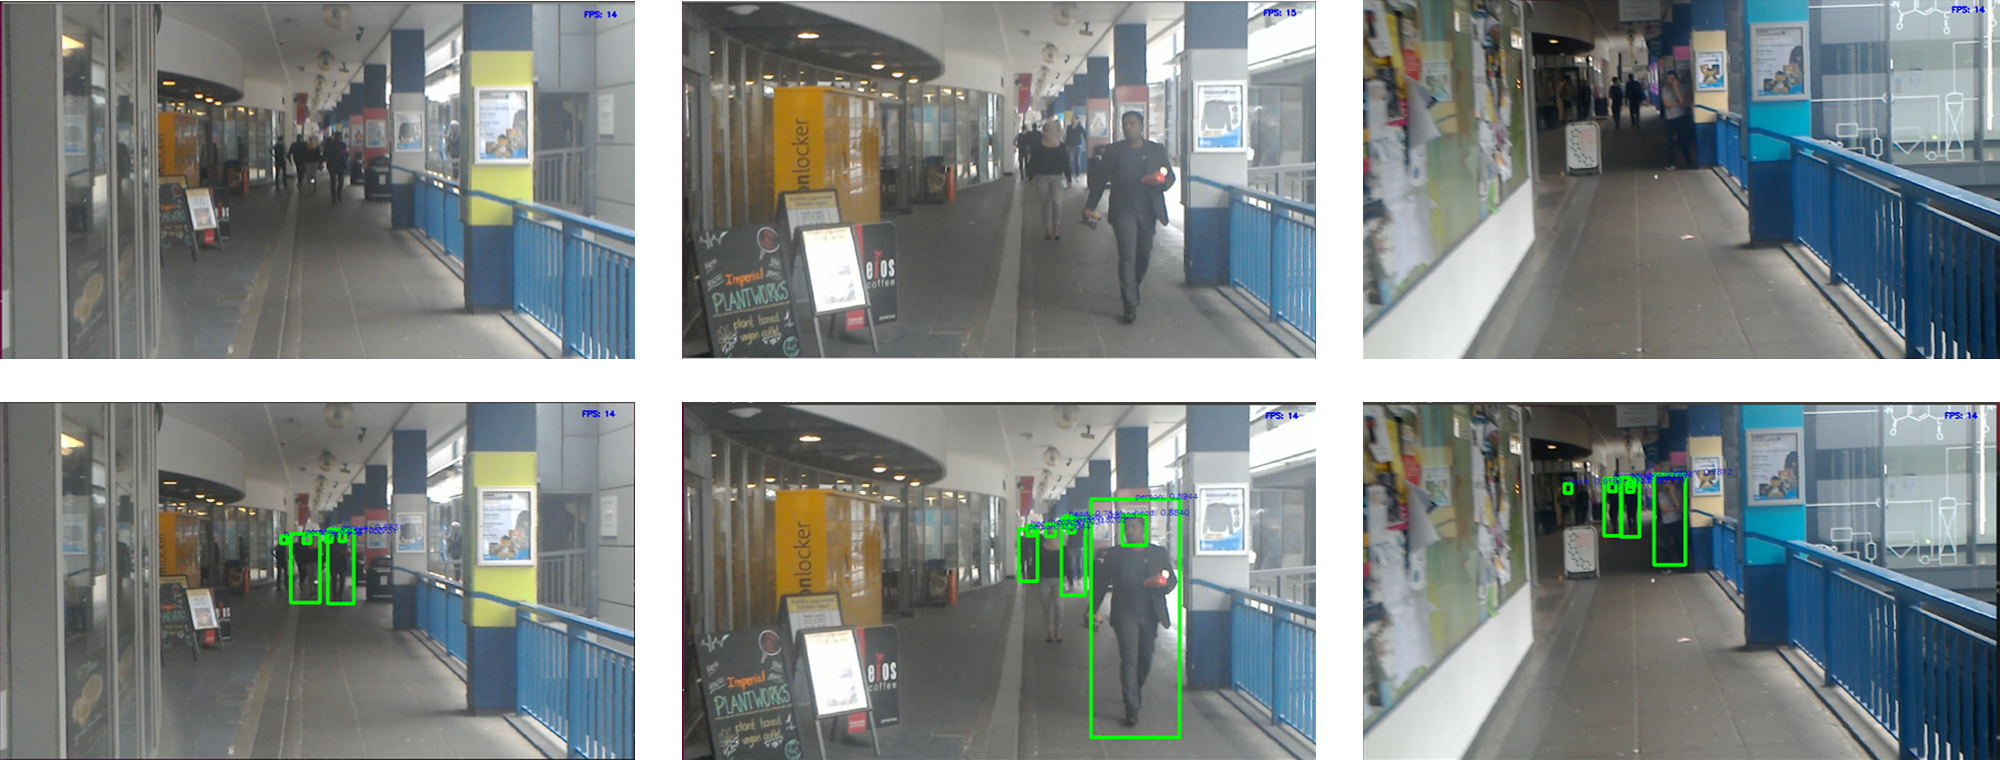
\includegraphics[width=0.95\linewidth]{img/chapter5_implementation/yoloWalkwayMultiple.png}
	\caption{Evaluating the model on Sherfield Walkway test video. We notice that it is able to small figures close together at a distance.}
	\label{fig:yoloSherfield}
\end{figure}

The videos from the Hololens were captured whilst a person was walking with the device, to best emulate a PWU in a wheelchair navigating through populated areas. We noticed an improvement in the number and accuracy of the detected bounding boxes compared with the pre-trained COCO models provided by Darknet. 



\subsubsection{ROS Node} \label{sec:nodeYOLO}
The Python wrappers for Darknet allow us to access the detection and image conversion functionality of the framework. To fully integrate the framework as a ROS node, we must follow the standard ROS procedures for creating a new ROS package. As such, we have created a package\footnote{https://github.com/alaksana96/fyp\_yolo} that runs Darknet and YOLO that can be downloaded and run seamlessly with ROS.

\paragraph{ROS Topics} The ROS node subscribes to the \code{/image\_transport/compressed} and expects to receive images in the compressed JPG format. This is because the Hololens captures video frames and encodes it to reduce the usage on the network bandwidth. These images are converted to numpy arrays which are further converted to Darknet \code{IMAGE} types for detection. 

\paragraph{} Darknet produces bounding box co-ordinates and class probabilities for each detection in an image. For every received frame, the node publishes the original image and a list of associated bounding boxes. The bounding box message contains the following information: \\

\begin{lstlisting}[language=Mymatlab,caption={BoundingBox.msg},label={bbmsg}]
string Class
float64 probability
int64 xmin % Top Left Corner
int64 ymin
int64 xmax % Bottom Right Corner
int64 ymax
\end{lstlisting}

\subsection{YACHT Package}
The major contribution of this project is in the form of the Yet Another Crowd Human Tracker package for ROS. This package utilizes the Deep SORT algorithm and OpenPose body pose estimation framework to attempt to determine the direction of individuals.


\paragraph{ROS Communication} As seen in Section \ref{sec:nodeYOLO}, the YOLO object detector node publishes a topic which contains the image and associated bounding boxes. Figure \ref{fig:detailedHL} shows that both YACHT nodes subscribe to the same output topic. The reason we decided to include the original image in the message and not just the bounding boxes is so that we can be sure the bounding boxes were detected for that frame, without having to subscribe to two seperate topics and comparing timestamps on individiual messages.

\subsection{YACHT: Tracker}
As explained in Section \ref{sec:YACHT}, the YACHT tracker depends on the Deep SORT algorithm \cite{Wojke2018}. Using the detections produced by the YOLO node, we assign IDs and match them across video frames to produce a track. These tracking IDs are then sent to the Hololens for visualization.


\subsubsection{Deep SORT} 



\paragraph{Modifications} We have modified\footnote{https://github.com/alaksana96/deep\_sort} Nicolai Wojke's original implementation of Deep SORT to run on Tensorflow-GPU. In the original, as the number of detections increased, so does the delay in tracking. This issue is more prevalent when tested on the MOT dataset, which has a large number of objects in each frame. Figure \ref{fig:deepSortCPU} visualizes the delay on the MOT16-06 video. We can see that the algorithm is operating at a very low FPS, causing it to be delayed in time. 

\begin{figure}[ht]
	\begin{subfigure}[b]{.45\textwidth}
		\centering
		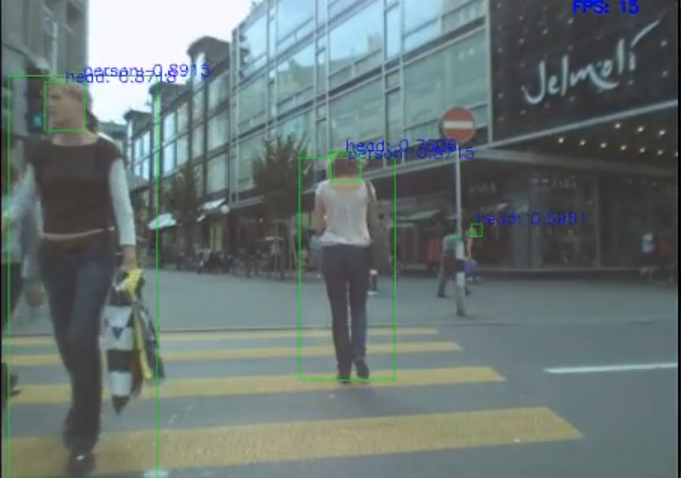
\includegraphics[width=1.0\linewidth]{img/chapter5_implementation/deepSortCPU.png}
		\caption{Output of YOLO. The image frame and bounding boxes are fed to Deep SORT}
	\end{subfigure}%
	\hspace{\fill} 
	\begin{subfigure}[b]{.45\textwidth}
		\centering
		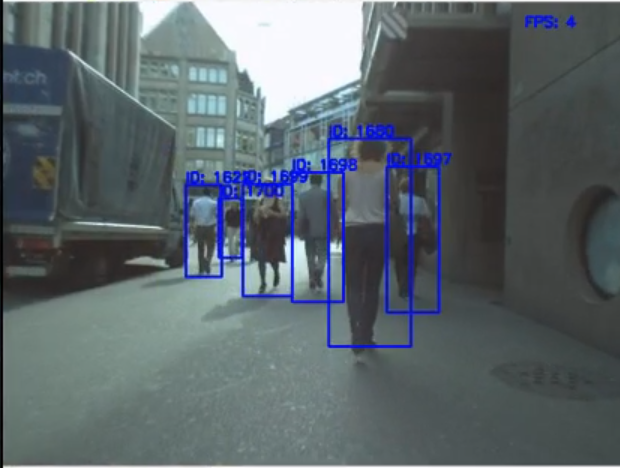
\includegraphics[width=0.935\linewidth]{img/chapter5_implementation/deepSortCPU1.png}
		\caption{Deep SORT is several frames behind since it runs at 4 FPS}
	\end{subfigure}
	\vspace{-1\baselineskip}
	\begin{center}
		\caption{Visualization of delay on CPU bound Deep SORT}
		\label{fig:deepSortCPU}
	\end{center}
\end{figure}


\paragraph{Deep Association Metric} Through code profiling, we noticed that the program was spending a lot of time in the generation of feature vectors. Upon inspection, we noticed that this process was run on a CPU bound version of Tensorflow. The \code{ImageEncoder} class uses a pre-trained deep network that generates the feature vectors for each bounding box. By using Tensorflow-gpu, we were able to run the network on system GPU, removing the delay. \\

\begin{lstlisting}[language=Python, caption={Deep SORT Tensorflow GPU modifications}]
class ImageEncoder(object):

	def __init__(self, checkpoint_filename, input_name="images",
				 output_name="features"):
				 
        # Tensorflow-GPU
        gpu_options = tf.GPUOptions(per_process_gpu_memory_fraction = 0.2)
        self.session = tf.Session(config=tf.ConfigProto(gpu_options=gpu_options))
\end{lstlisting}



\paragraph{Trackers \& Tracking} For each detection, we generate a feature vector using the image pixels within the bounding box. A matching cascade with Nearest Neighbour metric is used to best match the detection with existing confirmed tracks. Some detections will not get matched since the distance to confirmed tracks is above the \code{matching\ threshold}. The algorithm then attempts to match the detections to unconfirmed tracks using a simple Intersection-over-Union metric. These are newly created tracks that have existed for less than the last $n$ frames. If the detection is still unmatched, the algorithm creates a new tracker for the detection and adds it to the pool of unconfirmed tracks.

\begin{figure}[ht]
	\centering
	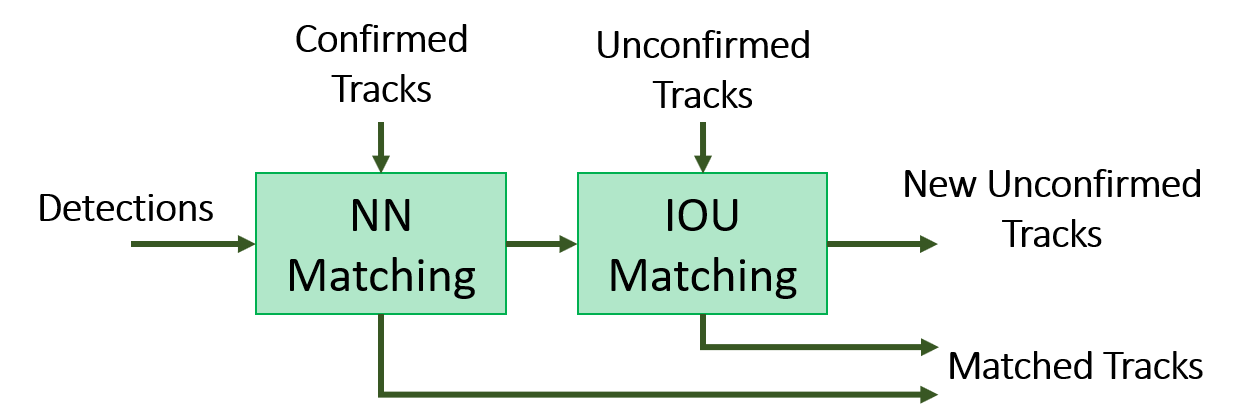
\includegraphics[width=0.8\linewidth]{img/chapter5_implementation/deepSortMatching.png}
	\caption{Visualization of Deep SORT matching. IOU matching is used as a final check for tracks that are unmatched by feature vector Nearest Neighbour matching.}
	\label{fig:deepSortMatch}
\end{figure}

Any pre-existing tracks which are not matched are checked. If the number of frames since the previous match is greater than the \code{max\_age} parameter, the track is considered dead and is deleted. This is done so as to prevent the number of tracks from growing infinitely. A Kalman filter is used to update the bounding box states of each track, as well as the time since the last update.
 
\subsubsection{Linear Extrapolation}
We experimented with linear extrapolation across frames as a way of inferring the direction travelled by the detection. As the project progressed, we encountered issues with this method, as explained in Section \ref{sec:objecTrackingDirection}. By searching for alternative methods, it was found that the depth camera on the Hololens can determine the distance between the PWU and an object relatively accurately. As such, we abandoned the pure computer vision approach in favour of using the Hololens.

\subsubsection{ROS Topic} \label{sec:yachtTrackROS}
The decision to use the Hololens depth cameras as a way of determining distance prompted the need for ROS messages to be sent to the device. As seen in Figure \ref{fig:detailedHDD}, the  tracker node publishes the bounding box and tracker ID to the Hololens. The \code{BoundingBox} data structure is defined in Listing \ref{bbmsg}, and is the same bounding boxes generated by the YOLO detector.

\begin{lstlisting}[language=Mymatlab,caption={ROS message structure for BoundingBoxID.msg}]
BoundingBox boundingBox
int64       id
\end{lstlisting}

\subsection{YACHT: Direction}
The second node in the YACHT package is the direction node, which uses the OpenPose framework to determine if a person is facing the camera or not. Earlier in Section \ref{des:YACHTBody}, we outlined the problem of not being able to determine the distance to an object with a regular pinhole camera model. We initially wanted to be able to determine the distance using only a video stream and computer vision techniques. However, we quickly realized that this was beyond the scope of the project, and decided to use the depth cameras on the Hololens.

\paragraph{} This section outlines the installation and setup of the OpenPose network \cite{Shao}. We also explain how we use the key-point detections to determine whether an individual is facing the PWU or not. Furthermore, we also explain how the bottom-up approach of OpenPose differs from the top-down approach that may have been more suitable, and the reasons for our implementation choices.

\subsubsection{OpenPose}
OpenPose is developed and maintained by the Carnegie Mellon University Perceptual Computing Lab. The implementation is made available on Github\footnote{https://github.com/CMU-Perceptual-Computing-Lab/openpose} to encourage body pose estimation research.

\paragraph{Installation \& Setup} The OpenPose library runs on a modified version of the convolutional neural network framework Caffe \cite{Jia}. The library is well documented, and provides its own instructions on how to setup the library. We direct the reader to the OpenPose GitHub repository if they wish to install the library themselves.

\paragraph{Model} As stated in Section \ref{des:body_25}, we use the \code{BODY\_25} keypoint estimation model for this project. The documentation states that this model is the fastest when it comes to real-time application, compared to the \code{MPI\_4} or \code{COCO} models. We also reduce the network resolution to $176\times 176$ to reduce the GPU usage and speed up the keypoint estimation. However, this reduces the accuracy of the detections, as discussed in this section.

\subsubsection{KeyPoint Estimation} \label{sec:bottomUp} 
Due to the bottom-up approach used by OpenPose, the network predicts key-points for individual body parts across the whole image. Through our testing on the MOT dataset, we noticed several points:

\begin{itemize}
	\item The model is good at detecting key-points of people close to the camera.
	\item People who are smaller and further away are not always detected.
	\item When people are close together or overlap, the keypoint estimation has difficulty differentiating between people.
	\item The more people in the image, the more network slows down and begins to lag behind the source video.
\end{itemize}

\begin{figure}[ht]
	\begin{subfigure}[b]{.32\textwidth}
		\centering
		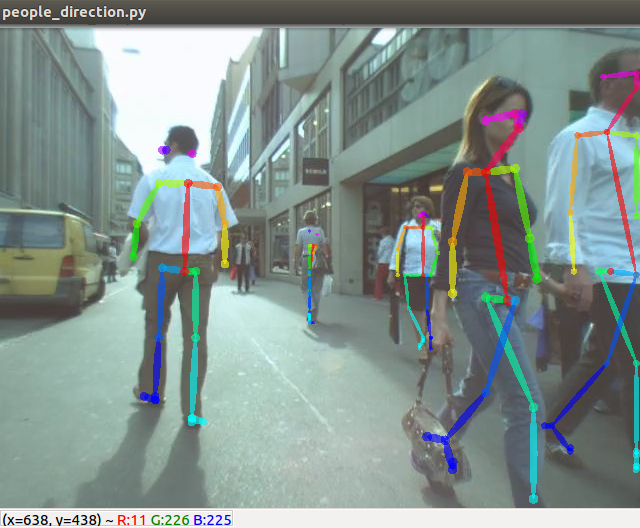
\includegraphics[width=1.0\linewidth]{img/chapter5_implementation/openposeKP.png}
		\caption{Key-point estimation is most accurate on people close-up.}
	\end{subfigure}%
	\hspace{\fill} 
	\begin{subfigure}[b]{.32\textwidth}
		\centering
		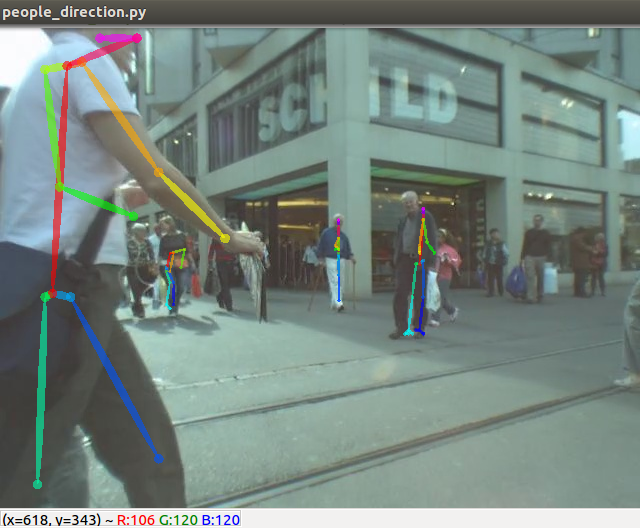
\includegraphics[width=1.0\linewidth]{img/chapter5_implementation/openposeKP1.png}
		\caption{On people at a distance, the estimation accuracy is limited by the network resolution.}
	\end{subfigure}
	\hspace{\fill} 
	\begin{subfigure}[b]{.32\textwidth}
		\centering
		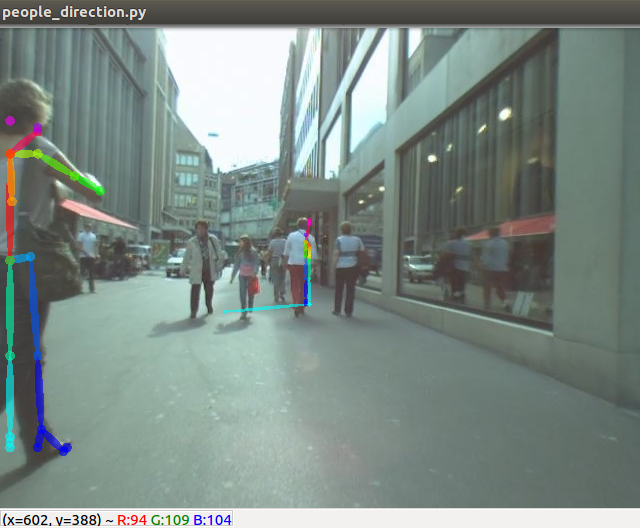
\includegraphics[width=1.0\linewidth]{img/chapter5_implementation/openposeKP2.png}
		\caption{A low network resolution results in difficulty discerning between people.}
	\end{subfigure}
	\vspace{-1\baselineskip}
	\begin{center}
		\caption{Comparison of keypoint estimation at different scales}
		\label{fig:openposeKP}
	\end{center}
		\vspace{-1.5\baselineskip}
\end{figure}

We highlight the issues in Figure \ref{fig:openposeKP}. The reason for the decrease in accuracy on people further away is due to the network resolution being lowered. Using a higher resolution allows us to detect people further away, but the delay between the arrival of the frame and the detection is more than 0.5 seconds. As such, to achieve real-time operation, we chose to use a lower network resolution.

\subsubsection{Defining Direction}
By comparing the relative positions of certain key-points, we can determine if a person is facing towards the camera or if they are walking away. This information is important, since it will allow for better visualization of where a person is walking, since people tend to walk in the direction they are facing. This also partially solves the direction problem brought up in Section \ref{sec:objecTrackingDirection}.

\begin{figure}[ht]
	\begin{subfigure}[b]{.32\textwidth}
		\centering
		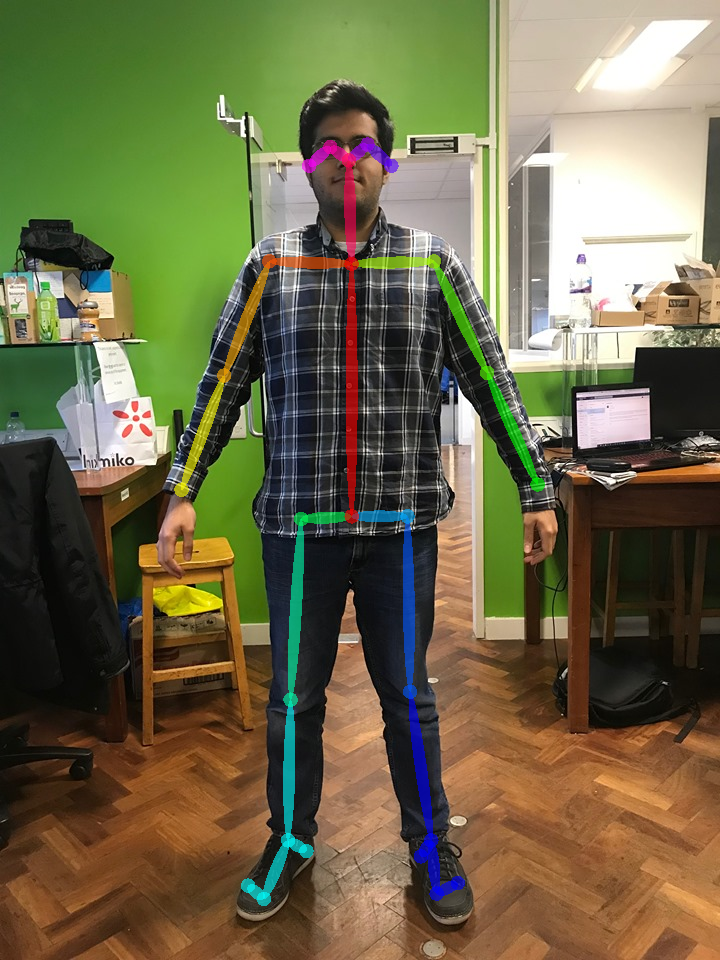
\includegraphics[width=1.0\linewidth]{img/chapter5_implementation/shreyFront.png}
		\caption{Frontal View}
	\end{subfigure}%
	\hspace{\fill} 
	\begin{subfigure}[b]{.32\textwidth}
		\centering
		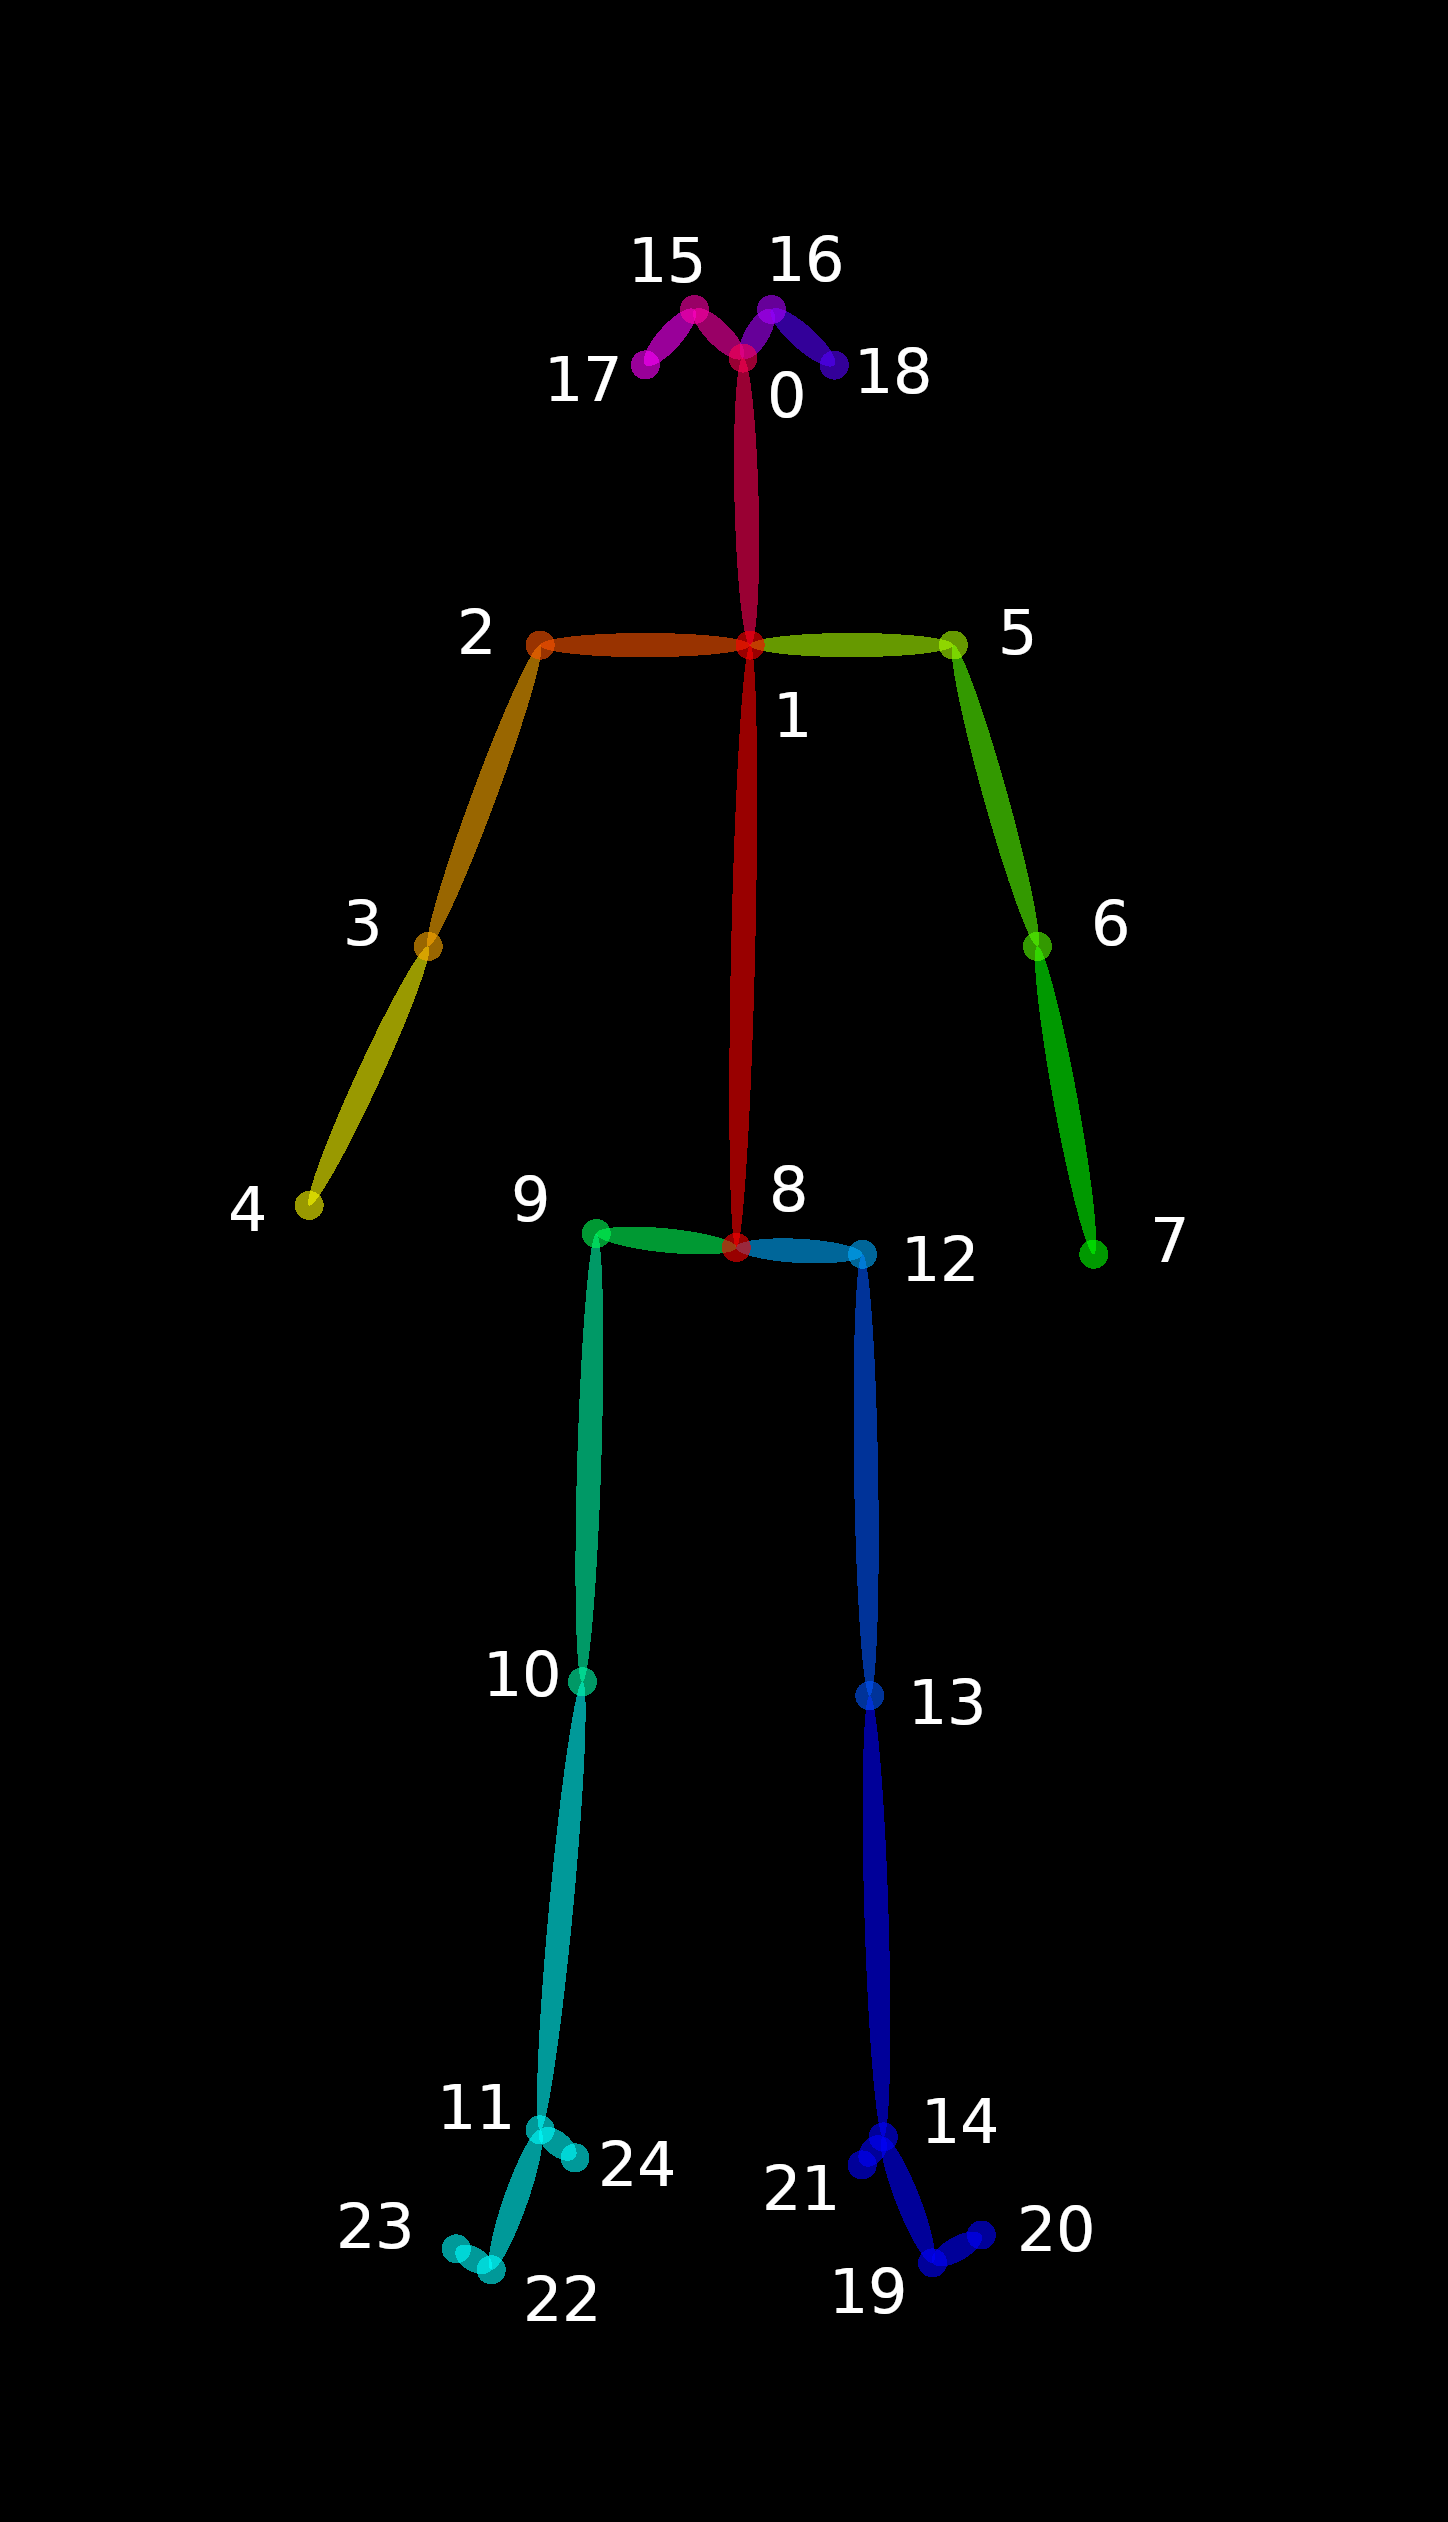
\includegraphics[width=0.765\linewidth]{img/chapter5_implementation/keypoints_pose_25.png}
		\caption{Key-point References}
	\end{subfigure}
	\hspace{\fill} 
	\begin{subfigure}[b]{.32\textwidth}
		\centering
		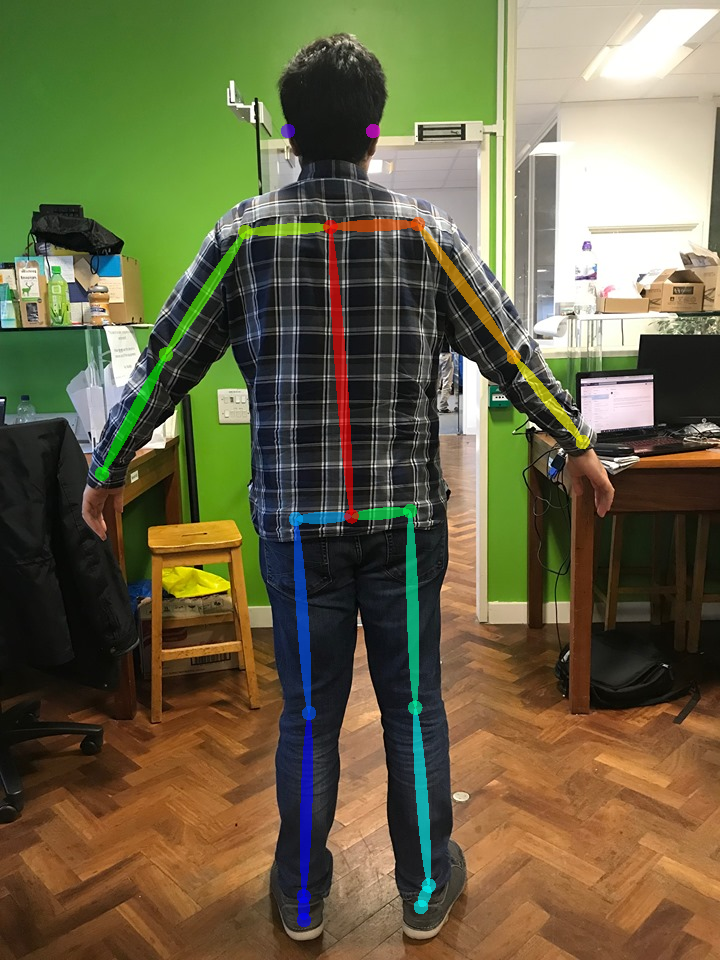
\includegraphics[width=1.0\linewidth]{img/chapter5_implementation/shreyBack.png}
		\caption{Back View}
	\end{subfigure}
	\vspace{-1\baselineskip}
	\begin{center}
		\caption{Body keypoint estimation of different views. These images show that the network can differentiate between left and right limbs.}
		\label{fig:keypointShrey}
	\end{center}
	\vspace{-2\baselineskip}
\end{figure}

\paragraph{Method} Pixels are measured from the top left corner of the image, with the x-axis extending horizontally to the right and the y-axis extending downwards. Figure \ref{fig:keypointShrey}.b shows the keypoint references for the body. The model is able to differentiate between the left and right limbs on a person. Figure \ref{fig:keypointShrey}.(a,c) show a full frontal and back keypoint detection on a person in the ideal detection position. 

\begin{table}[ht]
	\centering
	\begin{tabular}{|l|l|}
		\hline
		Body Part  & Key Points \\ \hline
		Right Arm  & 2, 3, 4    \\ \hline
		Left Arm   & 5, 6, 7    \\ \hline
		Head/Spine & 0, 1, 8    \\ \hline
	\end{tabular}
	\caption{Significant key-points for determining whether a person is facing the camera.}
	\label{tab:keypoints}
	\vspace{-1\baselineskip}
\end{table}

We can use the ability to differentiate between the left and right arms to determine if a person is facing the camera. Table \ref{tab:keypoints} presents the key-points for the relevant body parts. If the image co-ordinates of the left shoulder is further along the x-axis than the right shoulder, we can predict the direction as facing towards the camera. From testing, we know this simple method works most of the time. However, problems arise when a person is standing perpendicular to the camera. OpenPose has trouble detecting the torso and predicting the positions of the limbs, and it becomes difficult to decide if they are facing left or right.

\subsubsection{Implementation \& Detection Matching}
As mentioned in Section \ref{sec:bottomUp}, OpenPose uses a bottom-up approach by detecting individual body parts across the whole image. We need to match the OpenPose keypoint predictions with existing bounding boxes from YOLO, since these are assigned track IDs by the tracker node. This is done in Listing \ref{lst:matchDetPose} \\

\begin{lstlisting}[language=Python, caption={Direction and Detection Matching code in people\_direction.py}, label={lst:matchDetPose}]
def matchDetectionAndPose(self, detections, poses):
    for pose in poses:
        # Check torso, right/left shoulder
        torso, rshoulder, lshoulder = pose[1], pose[2], pose[5]

        for bbox in detections:
            if( self.withinBB(bbox, torso[0], torso[1]) or
                self.withinBB(bbox, rshoulder[0], rshoulder[1]) or
                self.withinBB(bbox, lshoulder[0], lshoulder[1])):
   
                if(rshoulder[0] > lshoulder[0]):
                    directionTowardsCamera = False
                else:
                    directionTowardsCamera = True

                publishDetectionDirection() 
                break # Once matched, move onto next pose 
\end{lstlisting}

\vspace{-1\baselineskip}

\subsubsection{ROS Topic} \label{sec:yachtDirROS}
The direction node publishes the bounding box and direction to the Hololens. The \code{BoundingBox} data structure is defined in Listing \ref{bbmsg}, and is the same bounding boxes generated by the YOLO detector. \\

\begin{lstlisting}[language=Mymatlab,caption={ROS message structure for BoundingBoxDirection.msg}]
BoundingBox boundingBox
bool        directionTowardsCamera
\end{lstlisting}

\newpage
\section{Hololens Unity Application}
The Hololens is the central device in the overall system, acting as an intermediary between the HDD system and ARTA. We rely on the AR capabilities of the device to render visualization holograms to indicate to the user potential collisions. The depth camera and other sensors are used to perceive the distance of detected objects which are communicated to ARTA for reactive assistance. Most importantly, the front facing camera is the main visual input for the whole system, beginning the whole image processing pipeline. Without a live video stream from the camera, object detection and direction inference would be impossible. As such, the initial phase of the project was dedicated to producing a reliable video stream to an external computer. Figure \ref{fig:detailedHololens} shows the two separate parts of the Hololens application, the camera stream and the holographic world. 

\begin{figure}[ht]
	\centering
	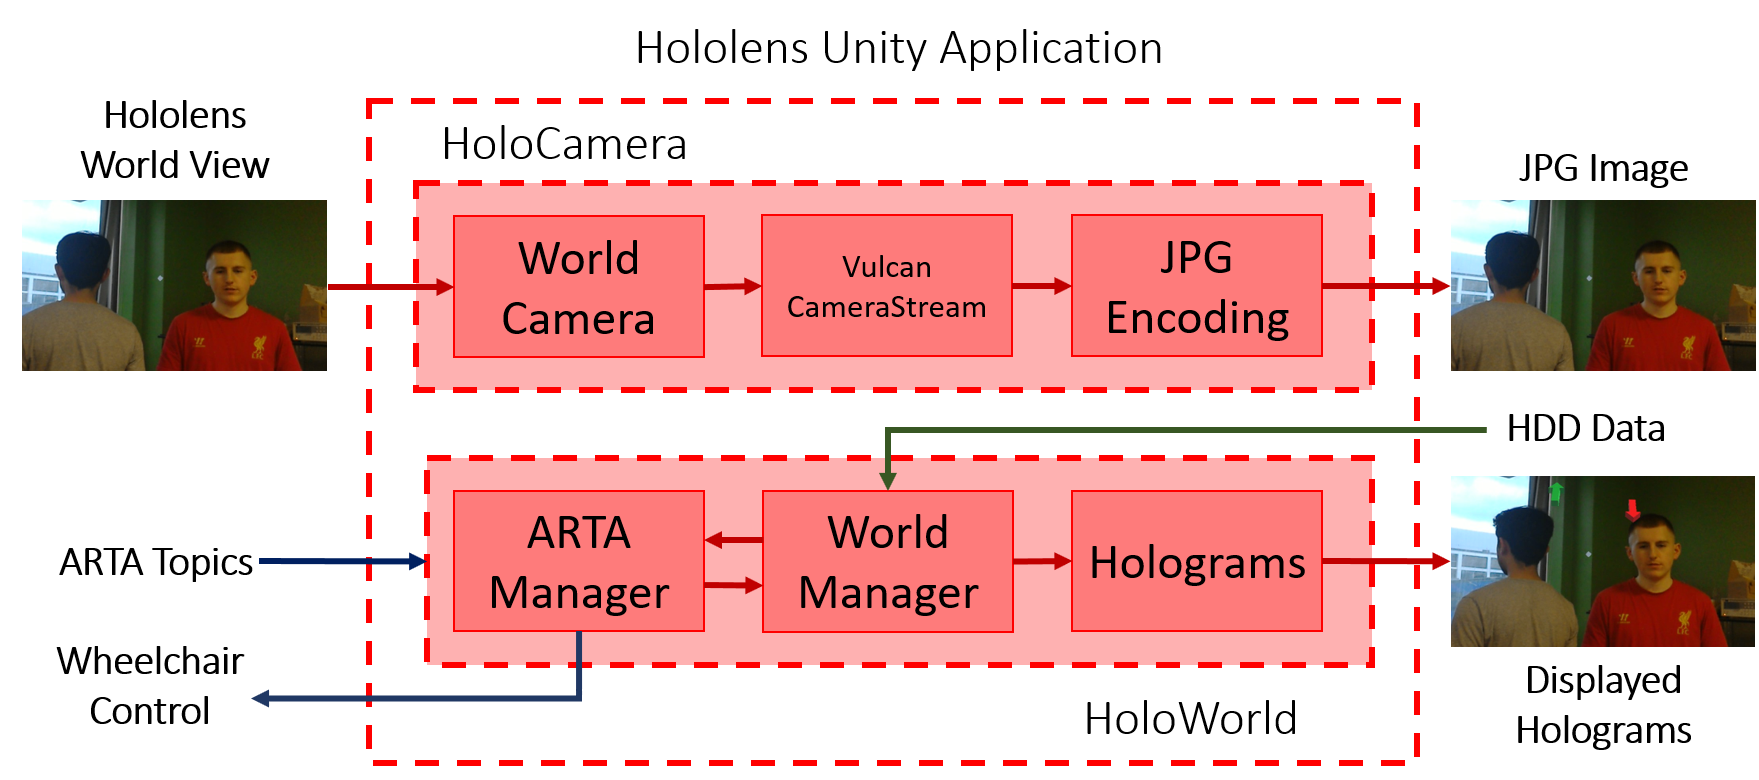
\includegraphics[width=1.0\linewidth]{img/chapter5_implementation/hololensSystemDiagram.png}
	\caption{Components of the Unity application running on the Hololens. We divide the program into two sub-programs, HoloCamera and HoloWorld.}
	\label{fig:detailedHololens}
\end{figure}

\paragraph{} Due to the importance, we begin this section by describing the implementation of the video camera stream. We explain the libraries used, the the workarounds required to produce the stream and the limitations of using a Unity based approach. Afterwards, we explain the Unity application responsible for producing holograms, positioning ARTA and how detected objects are placed in the Unity world. Finally, we explain the interaction between the Hololens and ARTA.

\subsection{Hardware \& Software Dependencies}
\subsubsection{Hardware}
\paragraph{Microsoft Hololens} The Microsoft Hololens is the world's first fully untethered holographic computer. The device has the ability to render 3D holograms in the world surrounding the user by displaying them on a set of see-through holographic lenses. The device is equipped with a multitude of sensors which we outlined in Section \ref{back:holo}. The device also supports gesture recognition for controlling the device, as well as voice input. The device is also able to connect to Wi-Fi networks, allowing it to stream data to and from other devices. We provide a complete device specification in the Appendix.

\begin{figure}[ht]
	\begin{subfigure}[b]{.45\textwidth}
		\centering
		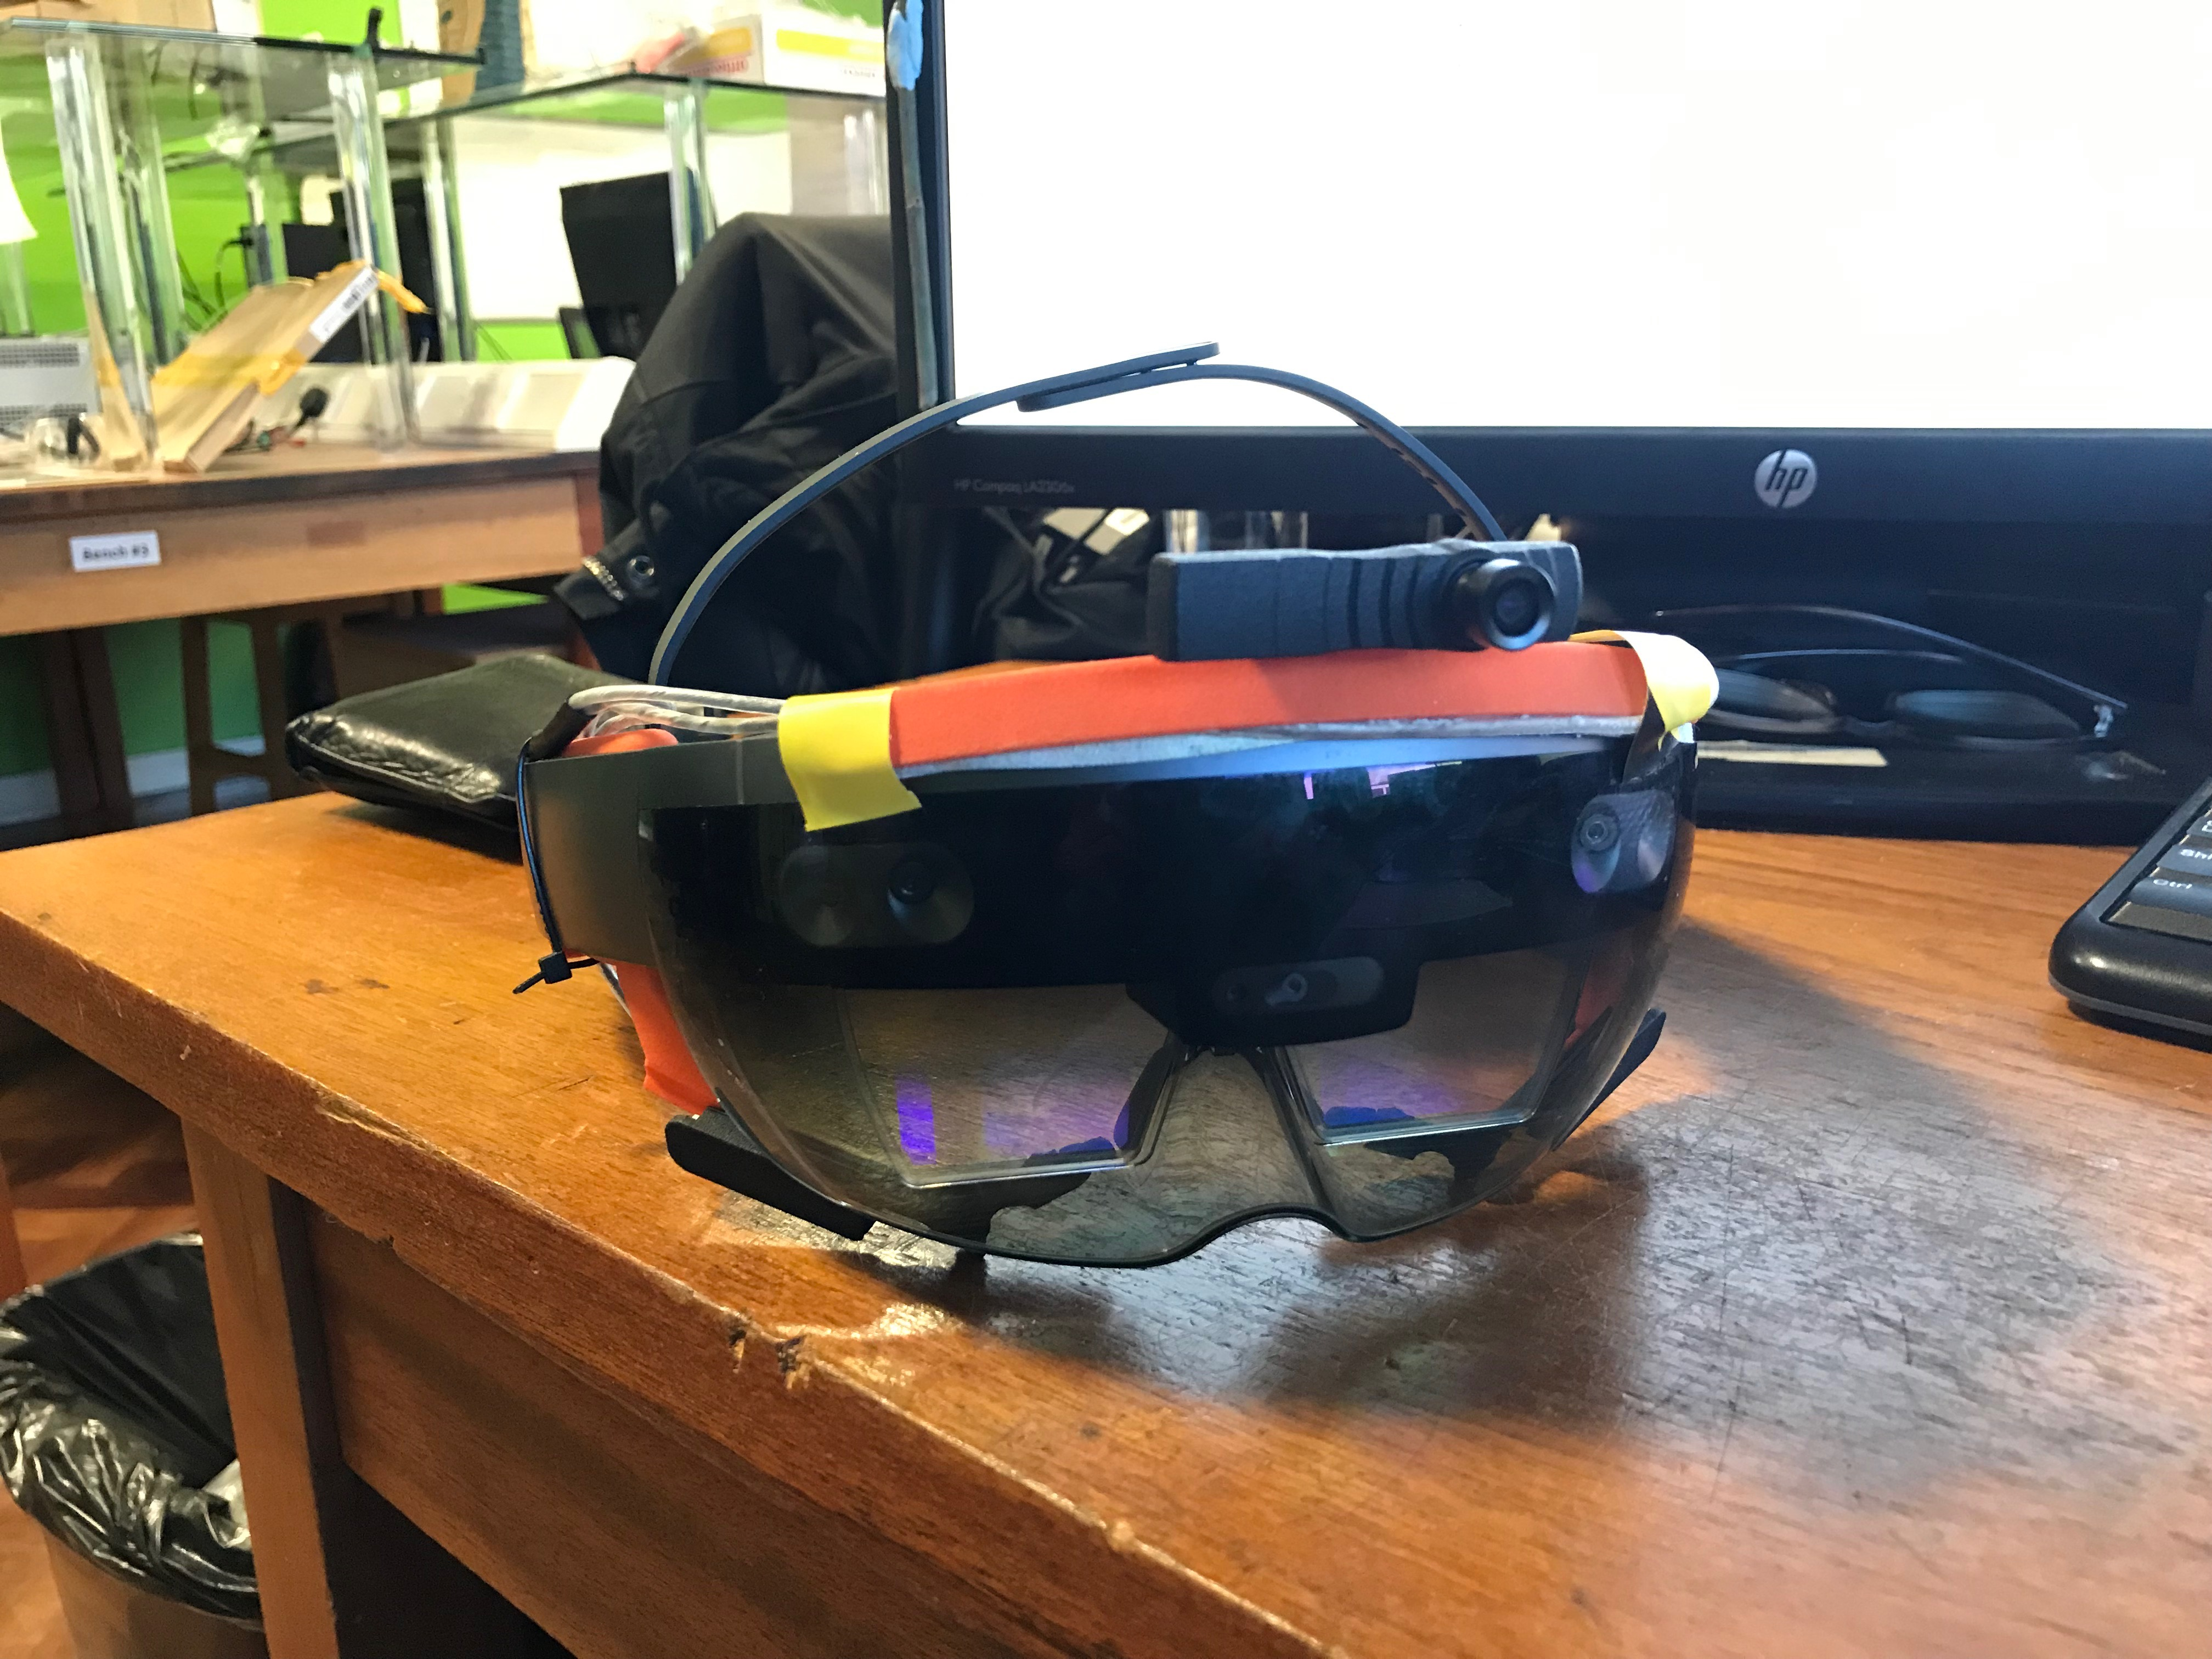
\includegraphics[width=1.0\linewidth]{img/chapter5_implementation/hololensDevice.jpg}
		\caption{The Microsoft Hololens with the see through holographic lenses.}
	\end{subfigure}%
	\hspace{\fill} 
	\begin{subfigure}[b]{.45\textwidth}
		\centering
		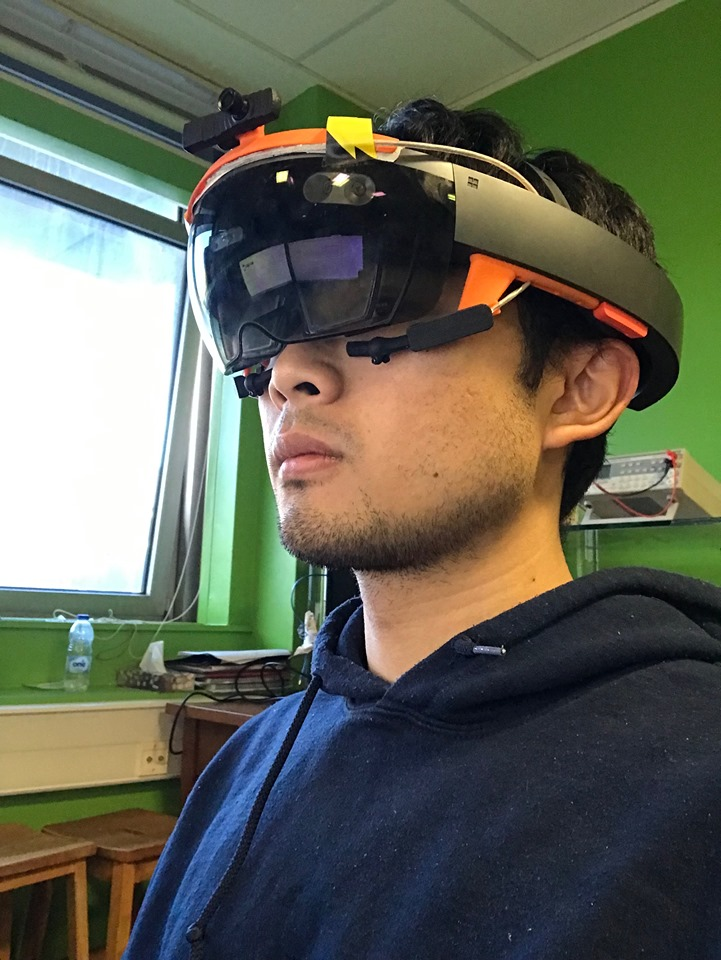
\includegraphics[width=0.55\linewidth]{img/chapter5_implementation/hololensOnHead.jpg}
		\caption{The device is worn on the head, resting on the bridge of the nose, similar to glasses.}
	\end{subfigure}
	\vspace{-1\baselineskip}
	\begin{center}
		\caption{The Hololens is larger compared to its competition. However, the increased number of sensors and wider spread usage makes it an ideal AR device for this project.}
		\label{fig:holodevice}
	\end{center}
	\vspace{-2\baselineskip}
\end{figure}

\subsubsection{Software}
\paragraph{Universal Windows Platform} The Universal Windows Platform (UWP) allows for applications that can be developed to run on any device running Windows 10. It gives the developer access to a set of standard APIs that make it easier to access data from any device. Software Development Kits (SDKs) are used to extend the capabilities of an app for specialized devices such as the Hololens.

\paragraph{Unity} Unity is a cross-platform game engine used to develop 3D, 2D VR \& AR visualizations for applications such as games, engineering or assistive robotics, among others. The main programming language for the engine is C\#, and the engine features built-in Windows Mixed Reality and Hololens support, allowing for easy development of applications for the Hololens. 

\paragraph{Development Tools} For this project, we used the following setup for development:

\begin{itemize}
	\item Microsoft Hololens running Windows 10
	\item Laptop running Windows 10 Developers Fall Edition
	\item Unity Editor 2018.1.6f1 (64-bit)
	\item Visual Studio 2017 Community Edition
\end{itemize}

The application produced in the Unity Editor and Visual Studio 2017 is compiled and deployed to the Hololens as a UWP Unity application that can be accessed and run from the device's heads up display menu.

\subsection{Hololens Locatable Camera}
The images captured by the front facing camera is meant to be a representation of what the user is seeing. In reality, the field of view (FOV) of the front facing camera is greater than the actual FOV of the device, meaning the camera can see more of the world than the user can. 

\subsubsection{Specifications}
The front facing camera is a 2 mega pixel photo/ HD video camera with auto white balance, auto exposure and a full image processing pipeline. Due to the real-time requirement of the project, we chose to use the smallest video resolution possible in order to achieve the fastest frame rates. This limits the resolution of the captured video frames to $896\times 504$.

\subsubsection{Limitations}
The greatest limitation of the Hololens is the field of view. The FOV of the front facing camera is 48 degrees wide, allowing it to capture images of the surrounding world. However, compared to a standard mobile phone camera, the front facing camera provides a cut-off view of the world. We highlight this issue in Figure \ref{fig:holoVsIphone}, which shows the reduced FOV of the device. Another issue is that despite the image processing the pipeline, the Hololens camera produces overexposed images, especially when the front facing camera is pointed towards illuminating objects or when light is only coming from one direction. 

\begin{figure}[ht]
	\begin{subfigure}[b]{.45\textwidth}
		\centering
		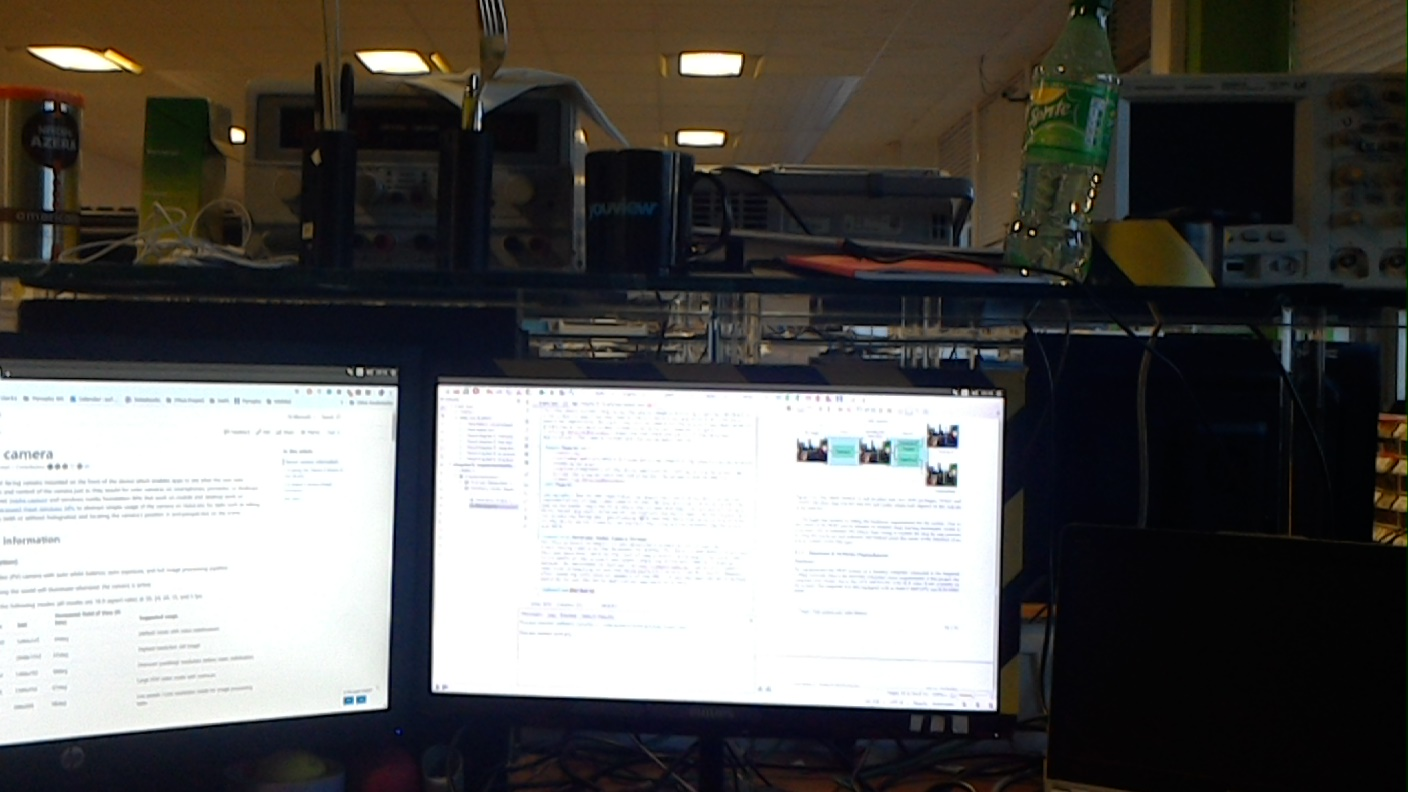
\includegraphics[width=1.0\linewidth]{img/chapter5_implementation/hololensFOV.jpeg}
		\caption{Image captured by Microsoft Hololens. Notice the overexposure in the image.}
	\end{subfigure}%
	\hspace{\fill} 
	\begin{subfigure}[b]{.45\textwidth}
		\centering
		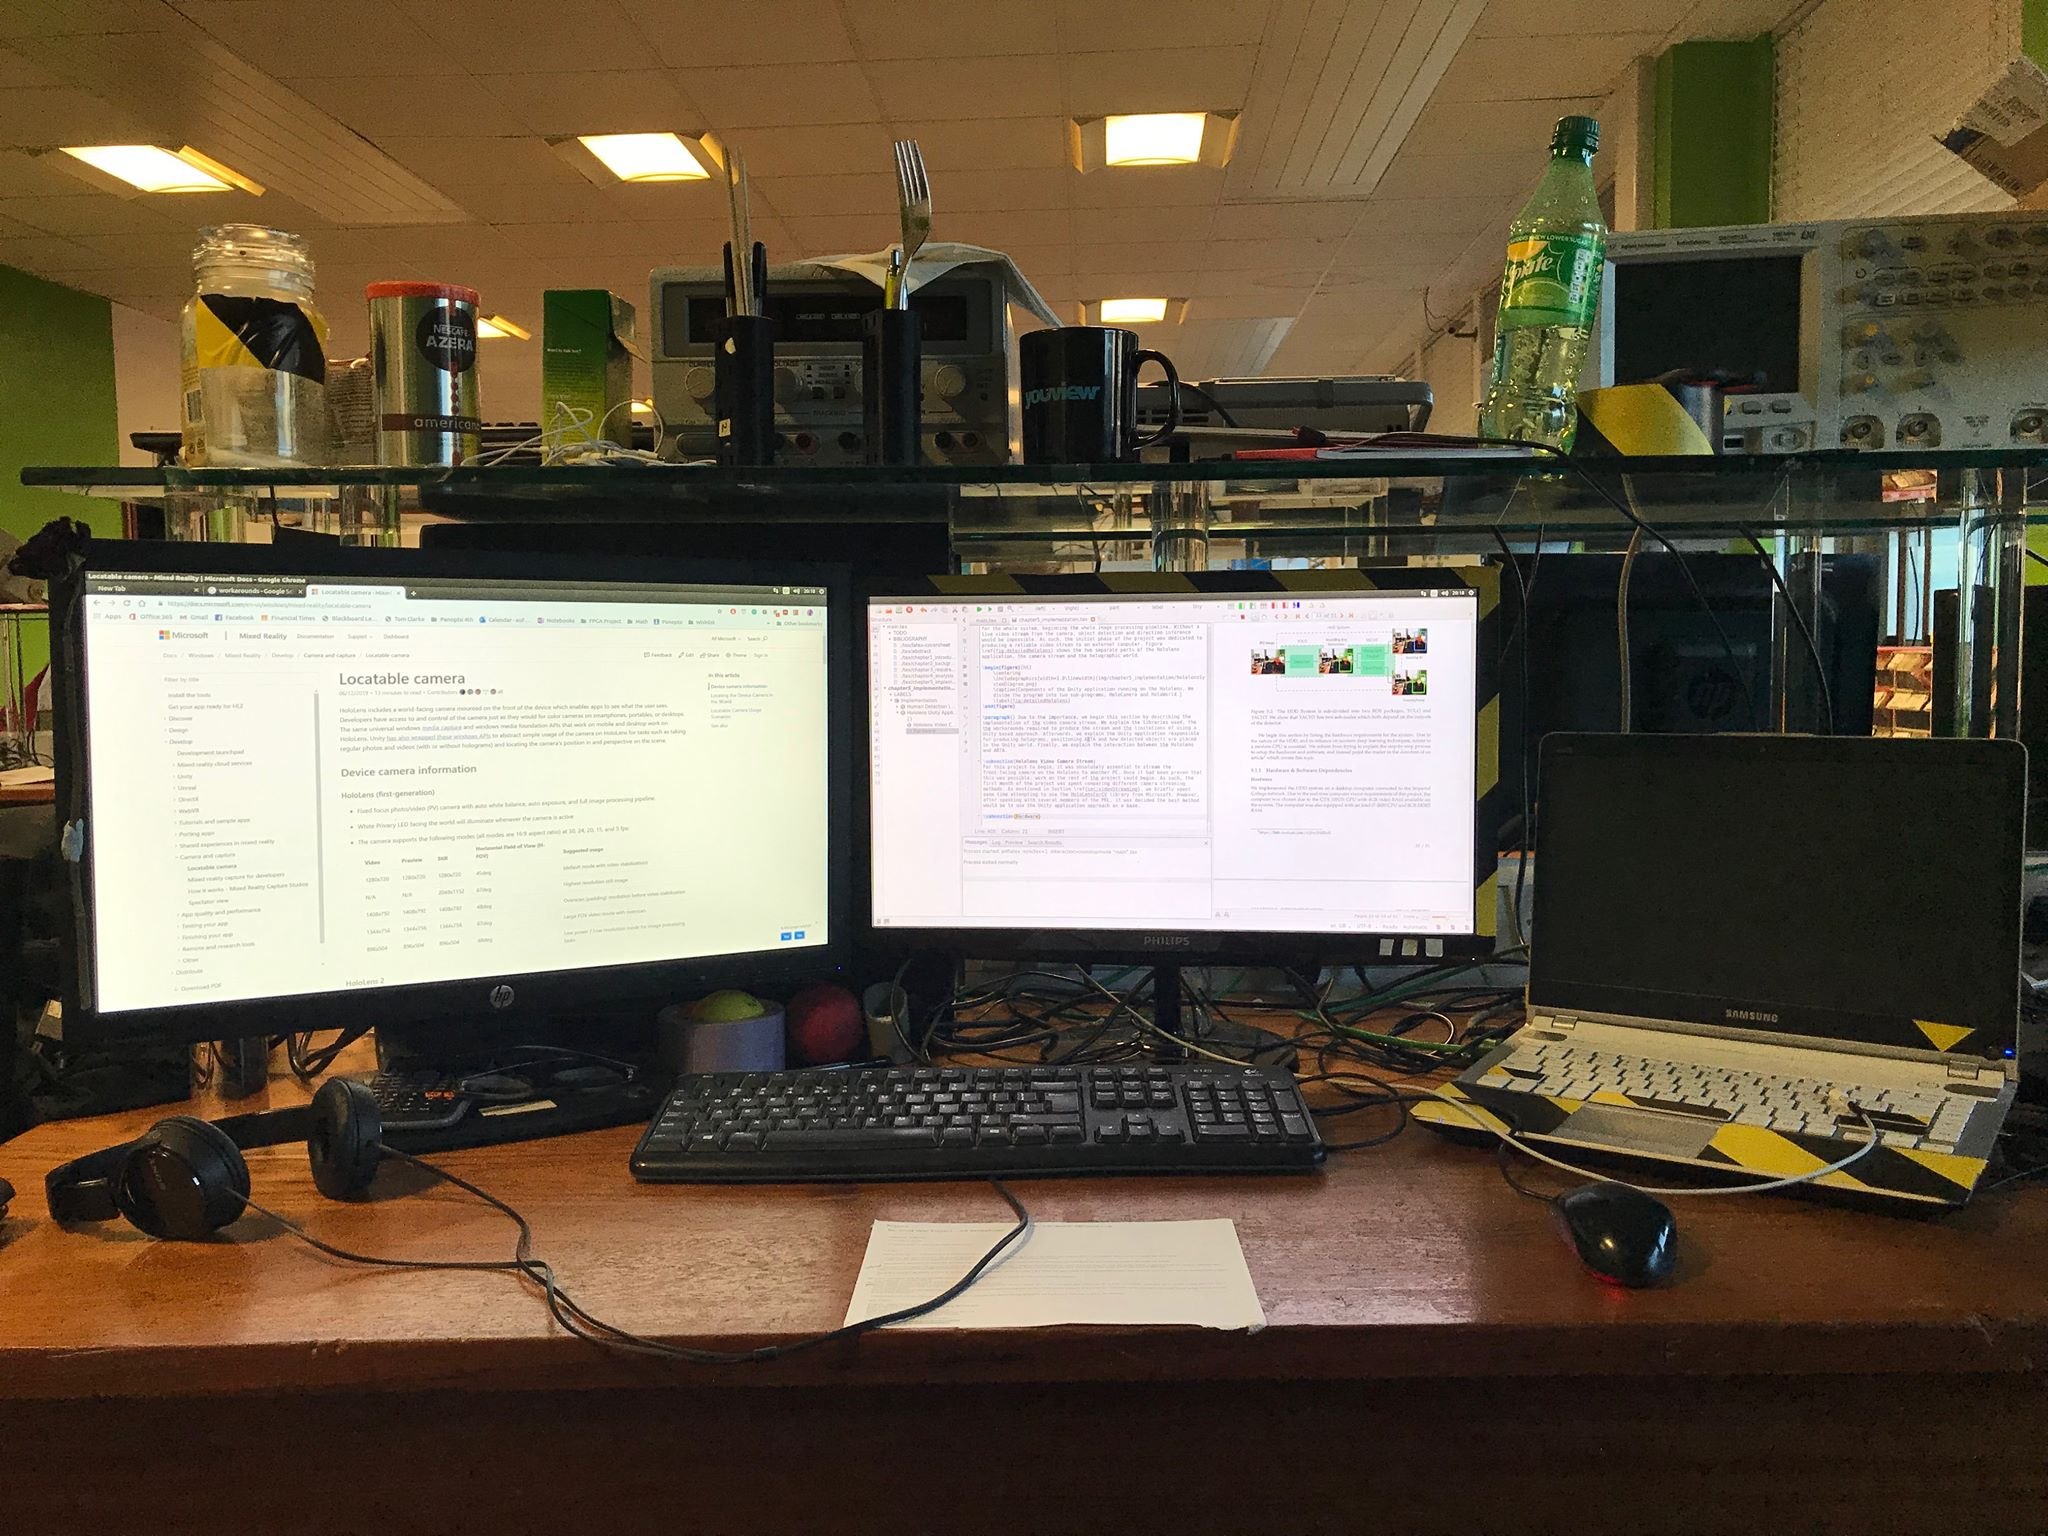
\includegraphics[width=0.75\linewidth]{img/chapter5_implementation/hololensFOVIphone.jpg}
		\caption{Image captured by standard IPhone Camera under the same light conditions.}
	\end{subfigure}
	\vspace{-1\baselineskip}
	\begin{center}
		\caption{These images were taken from the same position. The Hololens has a reduced FOV and is unable to capture the whole desk.}
		\label{fig:holoVsIphone}
	\end{center}
	\vspace{-2\baselineskip}
\end{figure}

Furthermore, due to the positioning of the holographic lenses, the users FOV is estimated to be approximately 29-30 degrees wide and 17 degrees high. This is even less than the front facing camera, and actually limits what the user can see in the surrounding area.

\subsection{Hololens Video Camera Stream}
For this project to begin, it was absolutely essential to stream the front-facing camera on the Hololens to another PC. Once it had been proven that this was possible, work on the rest of the project could begin. As such, the first month of the project was spent comparing different camera streaming methods. As mentioned in Section \ref{sec:videoStreaming}, we briefly spent some time attempting to use the HoloLensForCV library from Microsoft. However, after speaking with several members of the PRL, it was decided the best method would be to use the Unity application approach as a base.

\subsubsection{Image Capture}
The Unity engine on the Hololens has APIs for the front facing camera, giving developers access to information such as the resolution of the captured images, the camera intrinsics and the projection transform. However, Unity only allows developers to take a photo or video recording that is then saved onto the filesystem. The media can then be loaded from disk into Unity for streaming. This process is slow and time-consuming, due to the large overheads associated with writing media to and from disk. From experimentation, we deemed this method too slow for our use case, and sought out an alternative.

\paragraph{Vulcan Technologies} HoloLensCameraStream is a Unity plugin\footnote{https://github.com/VulcanTechnologies/HoloLensCameraStream} developed by Vulcan Technologies that makes the Hololens front facing camera frames available inside the Unity app in real time. The original library was developed to give developers the ability to show a preview of what the Hololens camera sees within the application. The ability to access the raw frames inside saves the application from having to write the frame to disk and loading it again. Unfortunately, the library has not been maintained for newer versions of Unity with the last stable version being Unity 2017.3.1f . Furthermore, these older versions of Unity are incompatible with the ROS\# library we use to communicate with other ROS nodes. As such, we updated the plugin for Unity 2018.1.6f1 by modifying offending code and updating obsolete functions to the newer 2018 Unity API.

\paragraph{Image Capture Pipeline} We briefly explain the image capture pipeline in the Unity application outlined in Figure \ref{fig:imgProcPipeline}. An instance of the updated Vulcan Technologies \textit{Camera Stream Helper} is added to the scene which provides access to the front facing camera video stream. We set the camera parameters to maximize the frame-rate by lowering the resolution. 

\begin{figure}[ht]
	\centering
	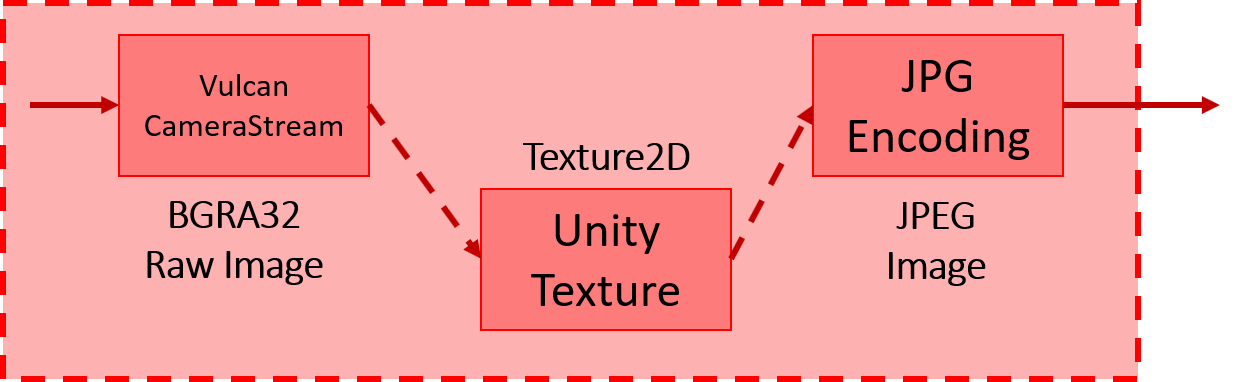
\includegraphics[width=0.6\linewidth]{img/chapter5_implementation/imageCapturePipeline.png}
	\caption{The image capture pipeline involves an intermediate Texture2D Unity state.}
	\label{fig:imgProcPipeline}
\end{figure}

\paragraph{} The captured frames are in the Microsoft standard \code{BGRA32} pixel format, which has 32 bits per pixel. The 4 channels (blue, green, red and alpha). are each allocated 8 bits per pixel. The raw pixel format creates large filesizes unsuitable for streaming over the network. As such, it becomes necessary to compress the images into a PNG or JPEG format. Unity has the ability to convert \textit{textures}, a data structure for rendering images inside applications into a compressed image format to be saved to disk. We leverage this ability to compress the raw BGRA32 bytes into a JPEG image ready for network transfer.

\subsubsection{Image Compression}
Unity has built-in image compression techniques for saving textures to disk. JPEG images are generated through a lossy compression technique. The degree of compression can be adjusted, allowing a trade-off between image quality and storage size. Since these images are to be streamed over the network, we want to limit the size of the files so as to not use too much bandwidth. On the other hand, we want the quality of the image to be high enough so that we can conduct image processing in the HDD system. Through experimentation, we chose to set the image quality to 50\%, the middle ground between quality and filesize.

\paragraph{Unity Threading} Applications running on the Unity engine support threading, but due to many Unity types not being threadsafe, certain actions must be done in the main thread of the application. The main thread is responsible for all object interactions in the scene, as well as the rendering of holograms and other visualizations. On the other hand, tasks such as image capture by the Vulcan Camera Stream can be done in separate threads which are switched to from the main thread. We visualize the threading process in Figure \ref{fig:unityThreads}.

\begin{figure}[ht]
	\centering
	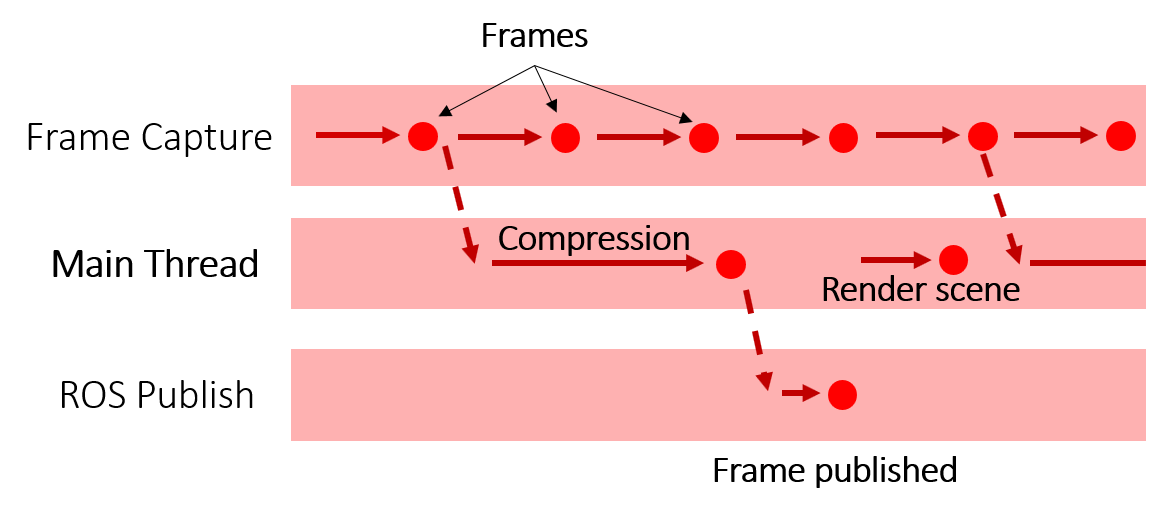
\includegraphics[width=0.8\linewidth]{img/chapter5_implementation/unityThreads.png}
	\caption{Image compression is a time consuming operation that must be done in the main thread. Only after compression is done can the holograms be rendered, limiting the application to 5 FPS.}
	\label{fig:unityThreads}
\end{figure}

\paragraph{Limited Frame-rate} An issue comes up with the way Unity implements image compression. The JPEG encoding reads the raw image bytes from a \code{Texture2D} object in the Unity scene. This action must be conducted on the main thread, since updating textures involves object interactions. From code profiling, we determined that it takes approximately $0.2$ seconds to compress a captured frame. As such, the rendering of the scene can only be done after image compression. This results in a slight latency of the visualizations viewed by the PWU. 

\subsection{ROS Communication}
As explained in Section \ref{sec:rossharp}, we use the ROS\# library originally released by Siemens for our Unity to ROS communications. However, the original ROS\# library was not developed for Unity applications running on UWP. As such, we used a variant of the library\footnote{https://github.com/dwhit/ros-sharp} developed by David Whitney, a PhD student at Brown University. 

\subsubsection{Modifications} The UWP version of ROS\# has been modified to only use APIs available on UWP devices such as the Hololens. Upon adding the ROS\# plugin to our Unity application, we encountered compatibility issues since the plugin was developed for Unity 2018.2 and above. We were forced to use 2018.1.6f1 since it is the most recent version of Unity where the HoloCameraStream library partially works, and it is possible to access the camera frames inside the Unity application. As such, we had to backport the ROS\# library by changing function calls to newer API features not available in our version of Unity.

\subsubsection{ROS Topics}

\begin{figure}[ht]
	\centering
	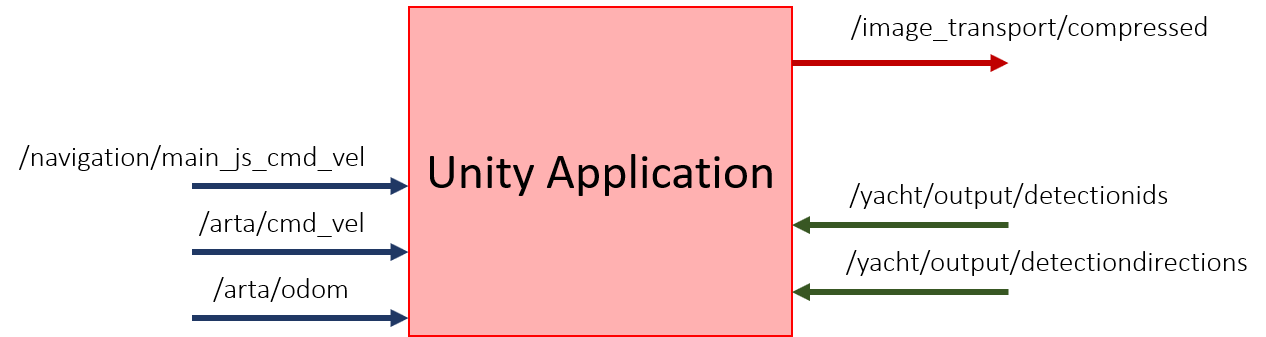
\includegraphics[width=1.0\linewidth]{img/chapter5_implementation/holoROSTopics.png}
	\caption{Image compression is a time consuming operation that must be done in the main thread. Only after compression is done can the holograms be rendered, limiting the application to 5 FPS.}
	\label{fig:unityThreads}
\end{figure}

\paragraph{Compressed Images} The raw video frames captured by the front facing camera are compressed into JPEG frames that can be published in the form of \code{CompressedImage} messages across ROS topics. Within the Unity application, we have setup \code{CompressedImage} publishers which are called when an compressed video frame is ready to be read into a message and published.

\paragraph{HDD Topics} In Section \ref{sec:yachtTrackROS} and Section \ref{sec:yachtDirROS}, we have explained the ROS messages published by the HDD system. The Hololens Unity application subscribes to these topics and receives the messages to transform the image co-ordinates into real world positions.

% TODO: TO ARTA


